\documentclass[a4paper, 12pt, openany]{book}

%% TIMES NEW ROMAN
\usepackage{newtxmath,newtxtext}

%% ARIAL
%\usepackage{helvet}
%\renewcommand{\familydefault}{\sfdefault}

\usepackage[ngerman]{babel}
\usepackage[a4paper, inner=2.5cm, outer=2.5cm, top=2.5cm, bottom=2cm, bindingoffset=0cm]{geometry}
%\usepackage[compact]{titlesec}
\usepackage{blindtext}
\usepackage{fancyhdr}
\usepackage{amsmath}
\usepackage{graphicx}
\usepackage{wrapfig}
\usepackage{amssymb}
\usepackage{xcolor}
\usepackage{etoolbox}
\usepackage{textcomp}
\usepackage{indentfirst}
\usepackage{chngcntr}
\usepackage{tabularx}
\usepackage{hyperref}
\usepackage{wrapfig}

% Authors
\usepackage{substr}
\usepackage[compact]{titlesec}
\newcommand\Chapter[2]{\chapter[#1 {\scriptsize\itshape#2}]{#1 \footnotesize\itshape#2}}
\newcommand\Section[2]{\section[#1 {\scriptsize\itshape#2}]{#1 \footnotesize\itshape#2}}
\newcommand\Subsection[2]{\subsection[#1 {\scriptsize\itshape#2}]{#1 \footnotesize\itshape#2}}
\newcommand\Subsubsection[2]{\Subsubsection[#1 {\scriptsize\itshape#2}]{#1 \footnotesize\itshape#2}}

% Chapter sizes
\titleformat{\chapter}[display]
{\normalfont\huge\bfseries}{\chaptertitlename\ \thechapter}{20pt}{\Huge}
\titlespacing*{\chapter}{0pt}{0pt}{40pt}

\RequirePackage[ngerman=ngerman-x-latest]{hyphsubst} % Fix: Silbentrennung

%\usepackage[hidelinks]{hyperref}
\hypersetup{colorlinks,breaklinks, allcolors=black, linkcolor=[RGB]{100,100,100}}

% UNICODE chars
\usepackage[T1]{fontenc}
\usepackage[utf8]{inputenc}

% Figure settings
\graphicspath{{figures/}}
\counterwithout{figure}{chapter}

% Cite cite cite
\usepackage{csquotes}
\usepackage[defernumbers=true,citestyle=verbose-ibid,giveninits=true,doi=false,eprint=false,isbn=false,autocite=footnote,backend=biber,citetracker=true]{biblatex}
\addbibresource{bib/ethik.bib}
\addbibresource{bib/misc.bib}
\addbibresource{bib/figures.bib}
\DeclareNameAlias{default}{family-given}
\DeclareDelimFormat[bib]{nametitledelim}{\addcolon\space} % Doppelpunkt nach Autor
\DeclareFieldFormat[article,inbook,incollection,inproceedings,patent,thesis,unpublished,techreport,misc,book]{title}{\mkbibquote{#1}}
\usepackage{fnpct}
\AdaptNoteOpt\footcite\multfootcite

% URL-Font normalisieren
\urlstyle{same}

\pagestyle{fancy}

\setlength{\headheight}{15pt} % Prävention der Warn-Nachricht

\fancypagestyle{plain} {
    \fancyhf{}
    \fancyhead[LE,LO]{Marvin Borner, Lars Krönner}
    \fancyhead[RE,RO]{Autonomes Fahren}
    \fancyfoot[CE,CO]{Seite \thepage}
    \renewcommand{\headrulewidth}{1pt}
    \renewcommand{\footrulewidth}{1pt}
}

\fancyhf{}
\fancyhead[LE,LO]{Marvin Borner, Lars Krönner}
\fancyhead[RE,RO]{Autonomes Fahren}
\fancyfoot[CE,CO]{Seite \thepage}
\renewcommand{\headrulewidth}{1pt}
\renewcommand{\footrulewidth}{1pt}

% \renewcommand{\footnotesize}{\fontsize{8pt}{10pt}\selectfont} % Footnote size
\renewcommand{\baselinestretch}{1.5} % 1.5 Linespacing

% Counter settings
\setcounter{tocdepth}{1}
\setcounter{figure}{0}

\pagenumbering{roman}
\begin{document}
    \titleformat{\chapter}[display]{\normalfont\bfseries}{}{0pt}{\huge}
    \titlespacing*{\chapter}{0pt}{-10pt}{20pt}

    \iffalse \title{%
        \Huge{\textbf{Autonomes Fahren\newline Autonome Fahrzeuge im moralischen Dilemma}} \\ % TODO: Besserer Titel (Autonome Fahrzeuge im moralischen Dilemma; oder so) 
        \vfill
        \large{
            Zum Thema: Zwiespältigkeit der Technik \\
            des Seminarkurses bei Herr Hönmann und Herr Ruoß
        }
        \author{Von Marvin Borner und Lars Krönner}
    
        \maketitle
    
        \pagebreak
    }\fi
    \begin{titlepage}
        \begin{center}
            \vspace*{1cm}
            
            \Huge
            \textbf{Autonomes Fahren}
            
            \vspace{0.5cm}
            \Large
            Autonome Fahrzeuge im moralischen Dilemma
            
            \vspace{1.5cm}
            \large
            \textbf{Von Marvin Borner und Lars Krönner}
            \vfill
            
            Zum Thema: Zwiespältigkeit der Technik\\
            des Seminarkurses bei Herr Hönmann und Herr Ruoß
            
            \vspace{0.8cm}
            
\includegraphics[width=0.4\textwidth]{rbs}
            
            %\Large
            Technisches Gymnasium\\
            Robert-Bosch-Schule Ulm\\
            08.06.2020
            
        \end{center}
    \end{titlepage}

    % \hspace{0pt}
    % \vfill\noindent
    % Hiermit erklären wir, dass wir die vorliegende Hausarbeit selbständig verfasst und keine anderen als die angegebenen Hilfsmittel verwendet haben.
    % Die Stellen der Hausarbeit, die anderen Quellen im Wortlaut oder dem Sinn nach entnommen wurden, sind durch Angaben der Herkunft kenntlich gemacht. 
    % Dies gilt auch für Zeichnungen, Skizzen, bildliche Darstellungen sowie für Quellen aus dem Internet.\newline\newline
    
    % \setlength{\tabcolsep}{48pt}
    % \begin{tabular}{l c r}
    %      & & \\ \hline
    %      Datum & Unterschrift & Unterschrift 
    % \end{tabular}{}
    % \setlength{\tabcolsep}{6pt}
    
    % \vfill
    % \hspace{0pt}
    % \pagebreak
    
    {
        \hypersetup{linkcolor=black}
        \tableofcontents
    }

    \Chapter{Einleitung}{Marvin Borner}
        Heutzutage sind schon circa 18\% der 18 bis 65-jährigen Deutschen bereit, sich ein autonomes Fahrzeug zu kaufen\footcite{statistagermans} und derzeitige Prognosen gehen von einer prozentualen Nutzung von autonomen Fahrzeugen gegenüber \enquote{normalen} Fahrzeugen in Europa bis 2030 von 13\% aus\footcite{statistaeurope}. Diese Zahlen zeigen uns schon heute, wie viel Potential in der Autonomie des Fahrens steckt und wie viele Personen bereits heutzutage bereit wären, dieses Potential zu fördern. Auch in den aktuellen Nachrichten und in den Gesetzesdiskussionen sieht man, wie sehr die Menschen und Politiker zu einer autonomen Navigation hinarbeiten. Diese Entwicklung sieht man unter anderem an der rapid steigenden Beliebtheit von Tesla, dem weltweit führenden Hersteller von autonomen Elektroautos, welcher derzeit auch eine neue \textit{Gigafactory} in der Nähe von Brandenburg plant\footcite{zeitgigafac} und somit die Welt der Autonomie ein Stückchen näher bringt. Dabei sind viele Dinge, wie die aktuelle Gesetzeslage, nicht ausreichend vorhandene Kartendaten, eine fehlende Akzeptanz bei Deutschen und viele durch die Autonomie auftretenden \hyperref[dilemmata]{ethischen Probleme} noch nicht vollständig geklärt und somit ein akutes Hindernis einer vollständigen Autonomisierung des Verkehrs. Dennoch gibt es in Teilen der Welt schon die nötigen Gesetze und teilweise sogar komplett autonom fahrende Taxis, welche viele Menschen täglich zu ihrer Arbeit bringen.\par
        Dabei stellt sich für viele Personen die Frage, wie solche Systeme zuverlässig funktionieren können und inwiefern eine sichere Beförderung von diesen garantiert werden kann. Des Weiteren kommen sehr viele Fragen zur Ethik und Moral und der konkreten Umgehung der ethischen Dilemma-Situationen auf. In dieser Seminararbeit wird sich deshalb mit ebendiesen auftretenden Fragen auseinandergesetzt und sowohl die Funktionsweise der technischen Aspekte, als auch die dadurch auftretenden Probleme weitestgehend analysiert.
    
    \pagenumbering{arabic}

    \iffalse
    \chapter{Aktuell}
        \Section{Gesetzeslage}
            Freiheit, Gleichheit, Brüderlichkeit
        \Section{Anderes... (Technik, Firmen, Gigafactory, ...?)}
            WUUP.
    \fi
        
    \chapter{Grundlagen}
        \Section{5 Stufen des autonomen Fahrens}{Lars Krönner}\label{5stufen}
            Um einen generellen Überblick sowohl für Fahrzeughersteller, als auch Fahrzeugführer, über das autonome Fahren und deren Arten zu schaffen, stellten sich verschiedene Wissenschaftler im Namen der \textit{NHTSA} (National Highway Traffic Safety Administration) der Herausforderung, fünf verschiedene Stufen der Automatisierung von Fahrzeugen und globale, für Firmen zu beachtende, Regeln zu definieren.\footcite[1--2]{national2013preliminary}
            
            \subsection*{Stufe 1}
                Zu der ersten Stufe (auch \enquote{Stufe 0} genannt\footcite[S. 4]{national2013preliminary}) werden ausschließlich diejenigen Fahrzeuge gezählt, welche bis auf insignifikante Assistenzsysteme, wie automatisch aktivierte Scheibenwischer, den Fahrer nicht weiter unterstützen. So hat ein derartiges Fahrzeug keine Möglichkeit, die Bremsen, Lenkung oder Geschwindigkeit zu beeinflussen und die vollkommene Kontrolle liegt allein beim Fahrer.\footcite[4]{national2013preliminary}
            \subsection*{Stufe 2}
                Fahrzeuge, die der zweiten Stufe zugeordnet werden, können mehrere unabhängig voneinander agierende Automatisierungssysteme besitzen, wobei die sichere Kontrolle des Fahrzeuges weiterhin beim Fahrer liegt.
                Derartige Systeme können beispielsweise den Fahrer bei bestimmten Aktionen wie der Spurhaltung unterstützen, oder auch im Sinne der Prävention von Unfällen die Lenkung oder die Beschleunigung beeinflussen.\footcite[4]{national2013preliminary}
            \subsection*{Stufe 3}
                Die dritte Stufe umfasst die Automatisierung von zwei parallel laufenden Steuersystemen, welche den Fahrer von der Steuerung entlasten sollen. Der Fahrer ist nach wie vor für die Überwachung der Fahrbahn und eine sichere Fahrweise verantwortlich und muss jederzeit für die Kontrolle verfügbar sein. Ein Beispiel für ein derartiges System ist ein adaptiver Tempomat in Kombination mit einer automatischen Fahrbahnzentrierung. Der Hauptunterschied zu der zweiten Stufe besteht also darin, dass das Fahrzeug der zweiten Stufe nicht zwingend auf die physische Anwesenheit des Fahrers angewiesen ist, da es die Kontrolle kurzzeitig auch alleine übernehmen kann.\footcite[5]{national2013preliminary}
            \subsection*{Stufe 4}
                Fahrzeuge mit diesem Automatisierungsgrad ermöglichen es dem Fahrer, die volle Kontrolle über alle sicherheitskritischen Funktionen unter bestimmten Verkehrs- oder Umweltbedingungen abzugeben und sich unter diesen Bedingungen stark auf das Fahrzeug zu verlassen, um Veränderungen dieser Bedingungen wahrnehmen zu können und bei der Notwendigkeit einer Interaktion dementsprechend die Kontrolle des Fahrzeuges wieder übernehmen zu müssen. Hierbei wird erwartet, dass der Fahrer gelegentlich und mit einer komfortablen Übergangszeit für die Kontrolle des Fahrzeuges zur Verfügung steht. Ein Beispiel dieser Stufe ist ein selbstfahrendes Fahrzeug, das feststellen kann, wenn und wann das System die Automatisierung nicht mehr übernehmen kann (beispielsweise bei schlechter sensorischer Umgebungswahrnehmung oder einem entgegenkommenden Baustellenbereich) und der Fahrer dementsprechend benachrichtigt wird, die Kontrolle wieder übernehmen zu müssen. Zusammenfassend beschreibt diese Stufe also im Vergleich zu den anderen Stufen ein Fahrzeug, das so konstruiert ist, dass vom Fahrer nicht zwingend erwartet wird, die Fahrbahn während der Fahrt zu überwachen.\footcite[5]{national2013preliminary}
            \subsection*{Stufe 5}
                Ein Fahrzeug der fünften und finalen Stufe ist so konzipiert, dass es alle sicherheitskritischen Fahrfunktionen selbständig ausführen kann und die Fahrbahnbedingungen während der gesamten Fahrt überwacht. Ein solches System sieht vor, dass der Fahrer Ziel- oder Navigationseingaben macht, von ihm aber keine durchgehende Aufmerksamkeit oder Fahrbereitschaft erwartet wird. Diese Stufe schließt somit sowohl besetzte als auch unbesetzte Fahrzeuge ein. Der Definition zufolge liegt die Aufgabe (und Garantie) des sicheren Betriebs ausschließlich beim automatisierten Fahrzeug selbst.\footcite[5]{national2013preliminary}\par
                \textit{Von dieser fünften Stufe ist in unserer ethischen und technischen Analyse auszugehen}.
            
    \chapter{Technische Aspekte}
        \Section{Sensorik}{Lars Krönner}
            Autonome Fahrzeuge erzielen durch \enquote{de[n] Einbezug von Sensormessungen in die Planung und Ausführung von Bewegungen}\footcite[60]{robotik} eine unter anderem auch unmittelbare Anpassung an Umweltsituationen. Diese Anpassung wird durch das Zusammenspiel verschiedener, meist redundant implementierter, Sensoren bewirkt, welche sowohl als Kombination von mehreren gleichen Sensoren (zum Beispiel mehreren Kameras), als auch als Kombination mehrerer verschiedener Sensorsysteme mit denselben Funktionen (zum Beispiel LiDAR und Ultraschall) vorkommen.\\
            
                Mithilfe des GPS (Global Positioning System) lässt sich die Position eines autonomen Fahrzeuges anhand der Längen- und Breitengrade auf der Erdkugel bestimmen. Die Position kann mithilfe weiterer Daten wie Beschleunigung, Höhenmeter und Geschwindigkeit weiter eingeschränkt werden.\footcite[37]{rathod2013autonomous} Diese Position wird sowohl für die autonome Navigation durch digitale Karten, als auch für die Kommunikation mit anderen Fahrzeugen (\hyperref[V2V]{Vehicle-to-Vehicle}) und Verkehrssystemen (\hyperref[V2I]{Vehicle-to-Infrastructure}) benötigt. Auch wenn höher automatisierte Systeme (Stufe 4 und 5) in der Theorie ohne Karten als Hilfe für deren Navigation auskommen könnten, ist ein Kartensystem dennoch in allen derzeitigen Systemen dieser Stufen integriert. Dies ist wichtig, da im Falle von Ausfällen der für die Navigation benötigten Sensorsysteme die Fahrzeuge auf die Navigation mittels Karten zurückgreifen können und somit die Sicherheit, zumindest für einen gewissen Zeitraum, bestehen bleibt.
            
                Basierend auf der Time of Flight (ToF) Technologie, welche eine genaue Ortung von Objekten, unabhängig von deren Reflektionsfähigkeit, ermöglicht\footcite{tof}, ist LiDAR (Light Detection and Ranging) eine Technologie, deren Sensoren es erlauben, in Echtzeit eine dreidimensionale Abbildung der $360^{\circ}$ - Umgebung zu erstellen, sowie die Identifizierung, Verfolgung und Erkennung von Objekten in diesem Bereich.\footcite{mooney2019lidar}\footcite[36]{rathod2013autonomous}
            
                Mithilfe von Ultraschallsensoren können, wie auch durch die LiDAR Sensoren, Objekte in der näheren Umgebung, wie zum Beispiel Bordsteine, erkannt werden und Abstände zu diesen gemessen werden.\footcite[37]{rathod2013autonomous}
                Ultraschall misst Distanzen zu Objekten mithilfe von Schallwellen beziehungsweise der Zeit, die diese benötigen, um von dem Sensor bis zu dem Objekt und wieder zurück zu gelangen.
                Im Allgemeinen ist Ultraschall eine sehr robuste und zuverlässige Technologie für Objekterkennung und Distanzmessung, welche unter fast allen Umständen einsetzbar ist.\footcite{ultrasonic}
                
                Radar (Radio Detection and Ranging) ist ein System zur Objekterkennung, welches unter Verwendung von Funkwellen die Entfernung, Höhe, Richtung und Geschwindigkeit von Objekten rund um das Fahrzeug herum messen kann.\footcite[37]{rathod2013autonomous}
                
                Mithilfe von Kameras wird ein meist dreidimensionales Bild der Front- und Heckumgebung erschaffen.\footcite[37]{rathod2013autonomous} Diese Bilddaten können durch ein \hyperref[dv]{neuronales Netz} ausgewertet werden, um Daten, wie zum Beispiel Verkehrsschilder oder Ampeln, aus den Bildern zu suchen und zu analysieren. 
                
                Um das System in einem sicheren Zustand zu halten, sind die Sensorsysteme redundant eingebaut. Diese Redundanz zeigt sich in mehreren Ausführungen: Manche Sensorsysteme sind nur mehrfach verbaut, andere Sensorsysteme hingegen überdecken sich in ihren Aufgaben und Einsatzmöglichkeiten. Dies führt dazu, dass falls ein Sensorsystem oder ein einzelner Sensor eines Sensorsystems ausfällt, das System (vorerst) in einem sicheren Zustand bestehen bleibt und somit das Unfallrisiko gering bleibt.  
                
                Als Beispiel für Sensorsysteme, deren Aufgaben sich überdecken, lassen sich LiDAR, Ultraschall und Radar betrachten. Diese drei Sensorsysteme haben die Aufgabe, Objekte im Umfeld des Fahrzeuges zu erkennen, einzuordnen und zu verfolgen. Dennoch ist es von großem Nutzen, alle diese Sensoren dauerhaft in die \hyperref[dv]{Datenverarbeitung} mit einfließen zu lassen, da dadurch fehlerhafte Sensorwerte einfacher erkannt werden können. Dies ist vor allem bei solch einem wichtigen Aufgabenbereich, wie dem dieser drei Sensorsysteme, wichtig.
                Abweichende Sensorwerte müssen nicht zwingend auf fehlerhafte Sensoren hinweisen, sondern können auch auf die Eigenheiten der verwendeten Sensorsysteme zurückzuführen sein.
                
                LiDAR etwa ist eine schnellere und noch genauere Technologie als Ultraschall, kommt aber dennoch unter manchen Wetterbedingungen wie Nebel oder Regen an ihre Grenzen, da das ausgesendete Licht dort gebrochen und/oder abgelenkt wird, wodurch die Messungen ungenau, wenn nicht vollständig unbrauchbar werden.\footcite[1695]{kutila2018automotive}
                
                Auch Messungen mit Ultraschallsensoren können Probleme aufweisen, da diese empfindlich auf Temperaturschwankungen reagieren und eine Oberfläche benötigen, welche den Schall gut reflektiert, damit präzise Werte gemessen werden können.
                
                In solchen Fällen, in denen ein Sensorsystem beeinträchtigt wird, muss in der Datenverarbeitung anhand von anderen Messwerten abgewogen werden, welcher dieser Werte verwendet wird.
                
        \Section{Kommunikation (V2X)}{Lars Krönner}
            Der Begriff V2X-Kommunikation fasst die beiden Bereiche der Kommunikation von autonomen Fahrzeugen zusammen: Kommunikation von Fahrzeugen untereinander (\hyperref[V2V]{V2V}) und die Kommunikation zwischen Fahrzeugen und Objekten der Verkehrsinfrastruktur (\hyperref[V2I]{V2I}).\footcite[3]{schmidt2008v2x} Die V2X-Kommunikation \enquote{hat als primäres Ziel [die Verkehrssicherheit] durch den Austausch von Informationen zu erhöhen}\footcite[3]{schmidt2008v2x}, dies wird durch eine Erweiterung des \textit{Wahrnehmungshorizonts} der autonomen Fahrzeuge erreicht: \enquote{Bisher ist dieser limitiert auf wenige hundert Meter, die der Fahrer direkt einsehen kann beziehungsweise bordeigene Sensoren beurteilen können}\footcite[1--15]{schmidt2008v2x}.
            Ein Beispiel hierfür stellt die folgende Grafik (\autoref{fig_v2com}) dar. Des Weiteren veranschaulicht diese Abbildung, mit welchen weiteren Systemen die Verkehrssysteme kommunizieren und wie dies ablaufen kann.
            
            \begin{figure}
                \centering
                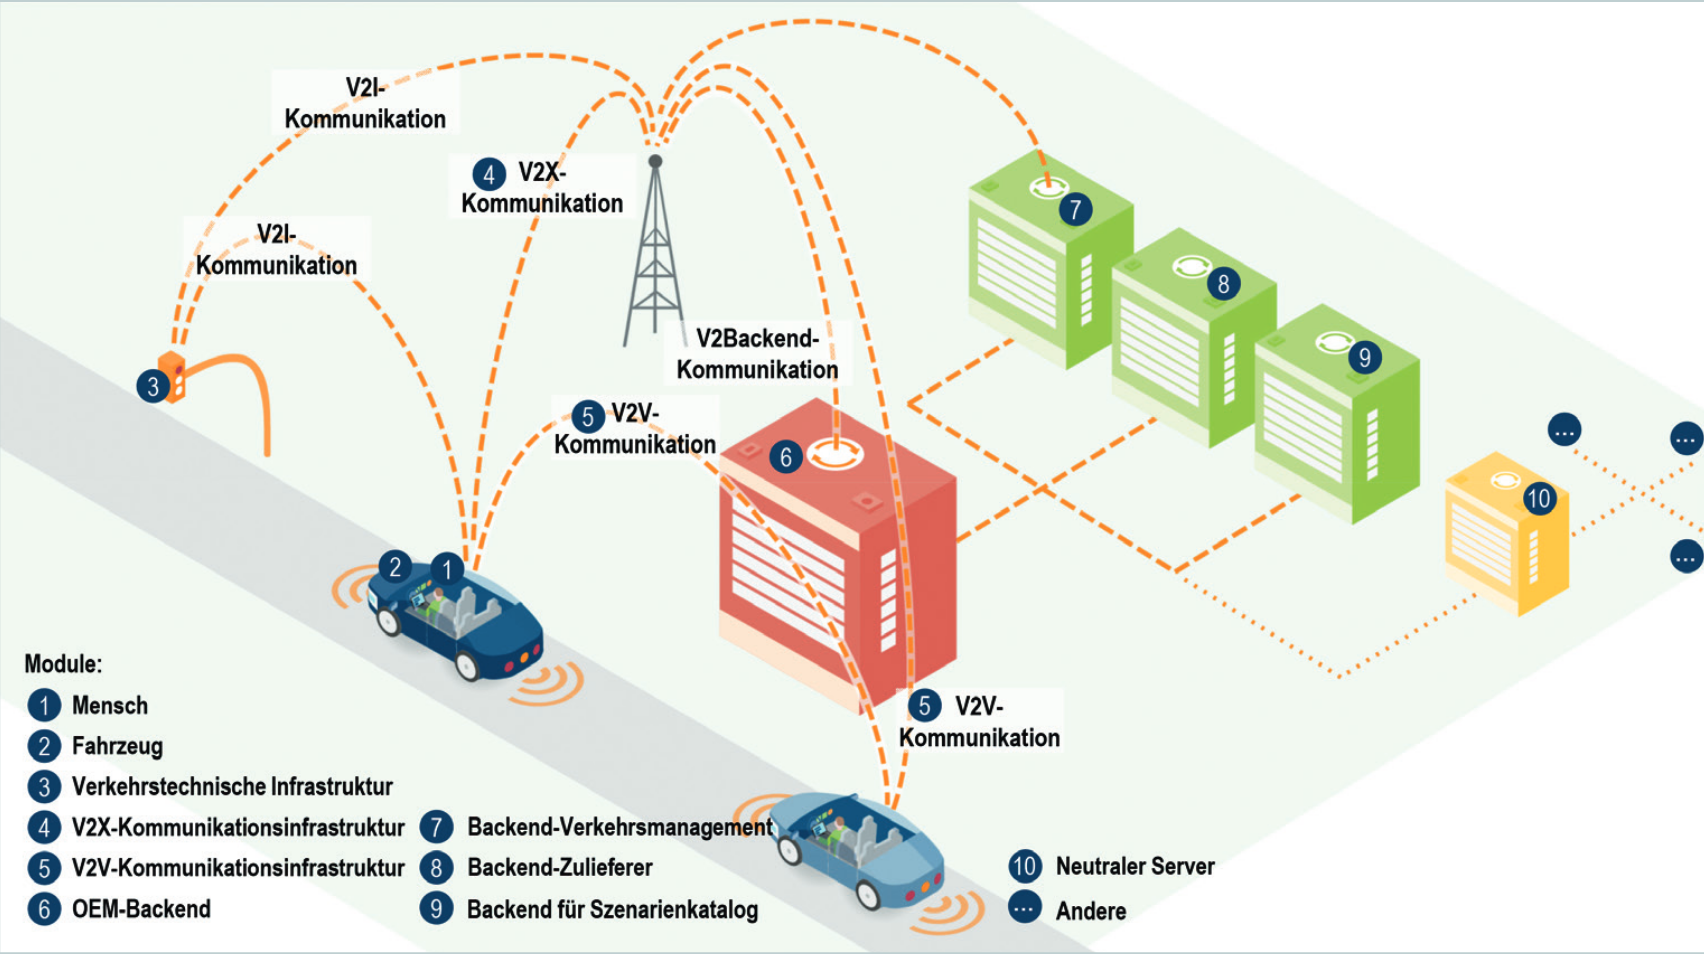
\includegraphics[scale=0.25]{v2wasauchimmer.png} 
                \caption{\cite{fig_v2com}}
                \label{fig_v2com}
            \end{figure}  
            
            Aus einer IT-Sicherheits-Perspektive betrachtet, müssen die Daten legitim und verlässlich sein, sowie eine dauerhafte Anonymität des Fahrzeuges gewährleistet sein. Um dies zu erreichen, muss es unmöglich sein, die übertragenen Daten zu manipulieren, das heißt in jeglicher Weise unechte Daten, wie imaginäre Unfälle oder Staus, in das System einzubringen. Zusätzlich dürfen die übertragenen Daten es nicht ermöglichen, nähere Informationen über den Besitzer des Fahrzeuges, wie Wohnort oder Arbeitsplatz, durch den Standortverlauf zu bekommen.\footcite{schmidt2008v2x}
            % https://sci-hub.se/https://ieeexplore.ieee.org/abstract/document/7355568
            % https://sci-hub.se/https://doi.org/10.1016/j.comnet.2011.03.016
            \subsection{Vehicle-to-Vehicle} \label{V2V}
                Die Vehicle-to-Vehicle (V2V) Kommunikation erlaubt es den damit ausgestatteten Fahrzeugen, Daten, wie Geschwindigkeit, Beschleunigung, Bremszustand, Standort und Fahrtrichtung, in einem circa 300 Meter großen Radius auszutauschen und sich somit ein Bild der näheren Umgebung zu schaffen.
                Die V2V Kommunikation basiert auf dem DSRC (Dedicated Short Range Communication) Protokoll, einem Funkprotokoll, welches speziell für die Kommunikation zwischen autonomen Fahrzeugen entwickelt wurde, und GPS.
                Durch die über das DSRC-Protokoll weitergegebenen Daten kann die Anzahl an Unfällen reduziert werden, da zum Beispiel Fahrzeuge andere Fahrzeuge in toten Winkeln erkennen können oder eine Weiterleitung von Nachrichten zwischen Fahrzeugen stattfinden kann, wenn beispielsweise ein Fahrzeug, welches sich nicht im Sichtfeld der eigenen Sensoren befindet, auf einer Autobahn abrupt abbremst.
                Bei der V2V Kommunikation werden bestenfalls jedoch keine Daten gesammelt und \textit{getrackt}, sowie keine für ein sicheres System unnötigen Daten weitergegeben, was ein großer Beitrag zum Thema Datenschutz ist.\footcite{nhtsav2v}
                
            \subsection{Vehicle-to-Infrastructure} \label{V2I}
                Die Vehicle-to-Infrastructure (V2I) Kommunikation fasst alle Arten der Kommunikation zwischen Fahrzeugen und Verkehrssystemen zusammen. Hierbei können mithilfe von Informationen der Infrastruktur Daten wie Informationen zu Baustellen oder Staus weitergegeben werden. Auch können durch den Internetzugang der Fahrzeuge Daten über größere Distanzen hinweg übertragen werden, obwohl dies nicht der Grundidee der V2X Kommunikation entspricht.\footcite[1--15]{schmidt2008v2x}
    
        \Section{Datenauswertung}{Lars Krönner} \label{dv}
            Durch die Messungen aller in den Fahrzeugen verbauten Sensorsystemen kommt eine große Anzahl an Daten zustande, welche in (fast) Echtzeit verarbeitet werden muss, sodass ein sicheres, autonomes Fahren in vollem Umfang zustande kommen kann.
            Die Verarbeitung dieser Masse an Daten kann durch neuronale Netze, besser bekannt als \textit{künstliche Intelligenz}, realisiert werden:
            \enquote{Diese Netze bieten sich überall dort an, wo [...] komplexe Beziehungen zwischen Eingabewerten (geliefert von Sensoren) und den in Abhängigkeit von diesen Werten zu steuernden Aktoren hergestellt werden müssen, oder wo [...] Strukturen in Daten erkannt werden müssen}\footcite[74]{robotik}.
            Diese Netze müssen in Fällen von sich stark unterscheidenden Messwerten der Sensoren, welche für dieselbe Aufgabe zuständig sind, entscheiden, welcher dieser Werte im jetzigen Zustand und der jetzigen Umgebung mehr Sinn ergibt. % Andere Formulierung
        
    
    \chapter{Ethik und Moral}
        Wie in den vorigen Kapiteln festgestellt wurde, sind Maschinen mit ihren Sensoren, der akkuraten Programmierung und der Fähigkeit, aus ihren eigenen Fehlern zu lernen, den Menschen inzwischen nicht mehr nur an Kraft und Präzision überlegen.\footcite[4]{birnbacher2016automatisiertes} Dennoch können Maschinen mit einer geringen, aber dennoch gewissen Wahrscheinlichkeit in kritische Situationen geraten, in denen sie schwierige Entscheidungen treffen müssen. \enquote{Ein Beispiel sind Dilemmasituationen, in denen schwere Schädigungen unvermeidbar sind und in denen die Maschine entscheiden muss, wie sie das Ausmaß des Schadens minimiert.}\footcite[4]{birnbacher2016automatisiertes} Derartige Entscheidungen werden besonders heute im Bereich des autonomen Fahrens sehr heftig diskutiert und bleiben leider oftmals ungelöst. In diesem Kapitel wird sich mit ebendiesen Diskussionen auseinandergesetzt und abschließend zu einer nahezu allumfassenden Lösung geführt, um die große Frage zu beantworten, ob autonome Fahrzeuge neben den gesetzlichen Vorschriften überhaupt moralisch vertretbar sein können.

        \Section{Ethische Dilemmata}{Marvin Borner} \label{dilemmata}
            \begin{quote} 
                \centering 
                \textit{\enquote{Der Fahrer eines Wagens fährt eine Straße am Hang entlang. Der vollautomatisierte Wagen erkennt,
                dass auf der Straße mehrere Kinder spielen. Ein eigenverantwortlicher Fahrer hätte jetzt die Wahl, sich
                selber das Leben zu nehmen, indem er über die Klippe fährt oder den Tod der Kinder in Kauf zu
                nehmen, indem er auf die im Straßenraum spielenden Kinder zusteuert. Bei einem vollautomatisierten Auto
                müsste der Programmierer oder die selbstlernende Maschine entscheiden, wie diese Situation geregelt werden
                soll.}\footcite[16]{ethikkommission}}
            \end{quote}\par
            Diese imaginäre Situation war das Thema einer langlebigen Diskussion der Ethik-Kommission des Bundesverkehrsministeriums Deutschlands. Hierbei ist festzuhalten, dass es sich um eine rein hypothetische Situation handelt und es keine Möglichkeit für die Kinder gibt, dem Fahrzeug auszuweichen, so wie es keine Möglichkeit für das Fahrzeug gibt, stehen zu bleiben. Die Kommission bekam den Auftrag, \enquote{die notwendigen ethischen Leitlinien für das automatisierte und vernetzte Fahren zu erarbeiten}\footcite[7]{ethikkommission}, um eine eindeutige und klare Lösung für die ethischen Schwierigkeiten zu finden, die autonome Fahrsysteme mit sich bringen.\par
            Wie sich herausstellte, gibt es keine derartige Lösung für die moralisch \textit{richtige} Entscheidung, sondern vielmehr verschiedene Ansätze und Gesetze, die angewandt werden können und somit zu unterschiedlichen Lösungen führen. Welche dieser Möglichkeiten dennoch die moralisch \textit{vertretbarste} Entscheidung ist, versuchten schon mehrere Philosophen zu entscheiden.
        
        \Section{Konsequentialistischer Ansatz}{Marvin Borner}
            Der Konsequentialismus beschreibt eine Herangehensweise an ethische Probleme, bei welcher die moralische Korrektheit einer Handlung abhängig von ihren Konsequenzen beurteilt wird.\footcite[133]{panza2011ethik}
            \subsection{Utilitarismus\footnote{Wenn in dieser Arbeit vom Utilitarismus gesprochen wird, ist der Handlungsutilitarismus gemeint.}}
                \enquote{Der Utilitarismus bestimmt den moralischen Wert einer Handlung anhand deren Auswirkungen}\footcite[221]{scholz2016autonomes} und ist somit eine Art des Konsequentialismus, welche den Nutzen beziehungsweise das Glück/Leid dieser Konsequenzen bewertet und die Handlung bevorzugt, die ein höheres Glück beziehungsweise kleineres Leid, folglich also einen höheren Nutzen, verursacht. Da die vollständige Betrachtung aller Konsequenzen einer Handlung nicht möglich ist (\enquote{Wie weit in die Zukunft soll man Konsequenzen betrachten?}), alleine weil der endlichen Menge an Ressourcen zufolge kein System jemals einen \enquote{unendlich großen Dateninput [im Sinne der Vorhersage] verarbeiten könne}\footcite[221]{scholz2016autonomes}, kann durch den Utilitarismus nie ein eindeutig klares Ergebnis gewonnen werden, sondern vielmehr eine gute Annäherung.\par
                Was wäre beispielsweise, wenn die Kinder eine Krankheit hätten und sowieso nur noch wenige Jahre leben würden? Oder sollte das Fahrzeug allein aus Autoritätsgründen die Kinder umbringen, wenn bekannt wäre, dass der Fahrer bald Präsident werden würde? Wenn derartige Fragen schon beim aktiven Wissen dieser Nebenfaktoren nahezu unmöglich zu beantworten sind, wie soll dann ein selbstfahrendes Fahrzeug alleine durch wenige Sensoren innerhalb weniger Sekunden evaluieren, was nun mehr Glück beziehungsweise Leid verursacht und somit \textit{gerechter} ist?\par
                Darüber hinaus widersprechen die Entscheidungen des Utilitarismus oft der moralischen Intuition.\footcite[221]{scholz2016autonomes} Wenn in einer etwas abgewandelten Situation die Straße beispielsweise eine zweischneidige Abzweigung wäre und auf der einen Seite die 90-jährige Großmutter des Fahrers stände und auf der anderen Seite ein dem Fahrer unbekannter Jugendlicher, dann würde sich der Fahrer vermutlich intuitiv dazu entscheiden, seine Großmutter zu schützen - auch wenn dem Utilitarismus zufolge der Jugendliche geschützt werden würde (längeres Leben $\Rightarrow$ weniger Leid und mehr Glück).
                
            \subsection{Hedonistisches Kalkül}
                Es fällt auf, dass der Utilitarismus keineswegs eine Lösung des Dilemmas bereitstellt, sondern nur eine gute Annäherung. Dies fiel auch dem Mitbegründer des Utilitarismus Jeremy Bentham auf und er entwickelte somit das Konzept des Hedonistischen Kalküls, mit welchem eine Aufrechnung des Glücks und Leids etwas präzisiert und einfacher durchgeführt werden kann. Ihm zufolge hängt die quantitative Größe des resultierenden Glücks beziehungsweise des Leids von mindestens vier Umständen ab:\footcite[105--106]{prechtl1995bentham}
                \begin{enumerate}
                    \item Intensität (Wie stark wird das Glück oder das Leid empfunden?)
                    \item Dauer (Wie lange dauert das Glück oder das Leid an?)
                    \item Gewissheit (Wie wahrscheinlich ist das entsprechende Resultat?)
                    \item Nähe (Wie weit liegt das Resultat in der Zukunft?)
                \end{enumerate}
                Durch dieses Kalkül kann das Glück und Leid einer Handlung bis auf Weiteres akkurat angenähert werden. In den folgenden Beispielen wird der Wert jedes Punktes jeweils zwischen $-5$ und $5$ gewählt, wobei eine negative Zahl für Leid und eine positive Zahl für Glück steht. Diese Analysen sind aufgrund der Definition und der fehlenden Klarheit der aus dem Kalkül folgenden Fragen rein subjektiv und können zwischen verschiedenen Menschen abweichen.

        \Section{Fallbeispiele}{Marvin Borner} % Inspiration: moral machine!
            Wie man an dem Beispiel der Ethik-Kommission sieht, sind derartige Dilemma-Situationen nicht einfach zu lösen. \enquote{Zur Bewältigung dieser Herausforderung erstellten wir [das MIT] ein Projekt namens Moral Machine [...] zur Erforschung der moralischen Dilemmata, mit denen autonome Fahrzeuge konfrontiert werden}\footcite[59]{awad2018moral}. Die Moral Machine ist eine Webseite, auf der möglichst viele Menschen die Entscheidungen von autonomen Fahrzeugen übernehmen beziehungsweise simulieren sollen, in dem sie zwischen zwei Möglichkeiten eine auswählen (\autoref{fig_moralmachine1}). Da die moralisch richtige Wahl beim autonomen Fahren eine direkte Korrelation zur durchschnittlichen Meinung aller Menschen haben kann, versucht das MIT mit diesem Projekt einen möglichst menschenähnlichen Entscheidungsalgorithmus zu entwickeln. \enquote{Diese Plattform sammelte 40 Millionen Entscheidungen in zehn Sprachen von Millionen von Menschen in 233 Ländern und Territorien}\footcite[59]{awad2018moral}. Dieses Projekt hat somit zu einer der umfangreichsten Analysen von moralischen Dilemma-Situationen in autonomen Fahrzeugen geführt.

            \subsection{Beispiel 1}
                \begin{figure}[h!]
                    \centering
                    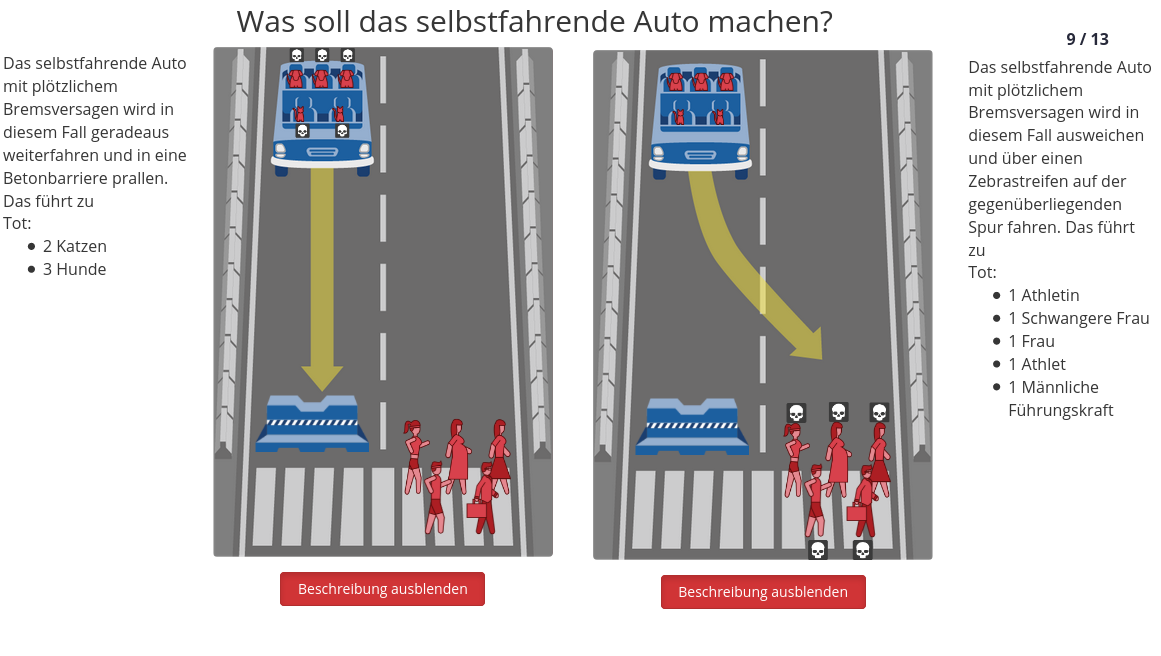
\includegraphics[scale=0.4]{mm1.png} 
                    \caption{\cite{fig_moralmachine1}}
                    \label{fig_moralmachine1}
                \end{figure}    
                    
                In \autoref{fig_moralmachine1} obliegt es dem voll-autonomen Fahrzeug der \hyperref[5stufen]{Stufe 5} zwischen dem Tod von fünf Tieren (linke Möglichkeit) und dem Tod von fünf Menschen (rechte Möglichkeit) zu entscheiden. Um eine utilitaristische Entscheidung zu treffen, muss nun das hedonistische Kalkül angewandt werden. Folgend wird in beiden Fällen jeweils das quantitative Leid berechnet und verglichen, um zu sehen, welche Handlung mehr Leid verursacht.

                \subsubsection*{Opfern der Tiere}
                    Da in diesem Beispiel keine Differenzen der Tiere bis auf deren Art beschrieben sind, können diese in der hedonistischen Analyse gleichgestellt werden. Für jedes Tier gilt demnach:
                    \begin{center}
                        \textbf{Fahrzeug fährt gegen die Absperrung: Tiere sterben}
                    \end{center}
                    \begin{center}
                        \begin{tabular}{|c|c|c|}
                            \hline
                            & Wert & Begründung \\
                            \hline
                            Intensität & -2 & Tod des Tieres \\
                            Dauer & -1 & Besitzende Person leidet \\
                            Gewissheit & -5 & Der Tod ist garantiert \\
                            Nähe & -5 & Geschieht direkt \\
                            \hline
                            Gesamt & -13 & \\
                            \hline
                        \end{tabular}
                    \end{center}\par
                    \vspace{.3cm}
                    Daraus ergibt sich ein Wert von $-13$. Prinzipiell wird also schon mal viel Leid erzeugt, was dem Utilitarismus zufolge generell für eine unmoralische Handlung spricht. Dieser Wert muss für das gesamte Fahrzeug mit fünf multipliziert werden, da sich fünf, hier gleichgestellte, Tiere im Fahrzeug befinden.
                    $$\Rightarrow -13 \cdot 5 = -65$$
                    Der Verlust des gesamten Fahrzeuges hat also einen moralischen Wert von $-65$. Eine konkrete Aussage zur moralischen Korrektheit kann dennoch erst getroffen werden, wenn dieser Wert von beiden Handlungen berechnet wurde. Hier fällt außerdem das vorher dargestellte Problem auf, dass es unmöglich ist, alle Hintergrundinformationen zu kennen. In diesem Fall beispielsweise, ob die Tiere überhaupt Besitzer haben und wie sehr diese leiden werden. In dieser Analyse wird von durchschnittlichen Haustieren ausgegangen, da mehr Informationen von der Moral Machine nicht gegeben wurden.
                
                \subsubsection*{Opfern der Menschen}
                    Zu den fünf Menschen, die in dieser Situation getötet werden sollen, gehören eine Athletin, ein Athlet, eine schwangere Frau, eine nicht näher spezifizierte, durchschnittliche Frau und eine männliche Führungskraft. Wenn es um das Ordnen der Wertigkeiten der Menschen geht, kann es zu Schwierigkeiten kommen. Im Allgemeinen sind im Utilitarismus alle Menschen gleichgestellt. Ist eine Athletin dennoch mehr Wert als eine normale, durchschnittliche Frau, weil sie einen gesünderen Lebensstil und somit auch eine längere Lebenserwartung hat? Dem Utilitarismus zufolge, ja, da ein längeres Leben grundsätzlich zu mehr Glück führt. Die Analyse mit dem hedonistischen Kalkül kann für einen durchschnittlichen Menschen deshalb so aussehen:
                    \begin{center}
                        \textbf{Fahrzeug fährt um die Absperrung herum: Menschen sterben}
                    \end{center}
                    \begin{center}
                        \begin{tabular}{|c|c|c|}
                            \hline
                            & Wert & Begründung \\
                            \hline
                            Intensität & -5 & Tod der Person \\
                            Dauer & -5 & Andere Personen leiden \\
                            Gewissheit & -5 & Der Tod ist garantiert \\
                            Nähe & -5 & Geschieht direkt \\
                            \hline
                            Gesamt & -20 & \\
                            \hline
                        \end{tabular}
                    \end{center}\par
                    \vspace{.3cm}
                    Der Einfachheit halber wird dieser Wert von $-20$ in diesem Kapitel als Standardwert eines durchschnittlichen Menschen gesehen und folglich nur noch mit Boni angepasst. Wenn man Frauen nun einen Bonus von $-3$ gibt, da diese mehr Glück durch Kinder bringen und im Durchschnitt länger leben\footcite[3]{lampert2014soziale}, einem sportlichen Menschen aufgrund seiner längeren Lebenserwartung\footcite[70]{gola2005adipositas} einen Bonus von $-2$, einer schwangeren Frau einen Bonus von $-5$ und der männlichen Führungskraft aufgrund der Jobs der Untergeordneten ebenfalls einen Bonus von $-3$ gibt, kommt man zu der Rechnung:
                    $$\Rightarrow (a - 3 - 2) + (b - 3 - 5) + (c - 3) + (d - 2) + (e - 3) = -121$$
                    Die Variablen sind hier nach der Reihenfolge der Personen in \autoref{fig_moralmachine1} benannt und haben jeweils den zuvor berechneten Wert von $-20$.
                
                \subsubsection*{Ergebnis}
                    Aus den vorherigen Analysen mit dem hedonistischen Kalkül ergibt sich somit, dass die rechte Handlung unmoralischer wäre als die linke, da das Opfern der Tiere einen gesamten moralischen Wert von $-65$ hat, das Opfern der Menschen jedoch $-121$, sprich mehr Leid verursacht. Dem Utilitarismus zufolge müssten demnach die Tiere geopfert werden. Selbstverständlich ist hier erneut festzuhalten, dass die Werte nicht genau bestimmt werden können und nach rein subjektivem Empfinden gewählt wurden.
            
            \subsection{Beispiel 2}
                \begin{figure}[ht!]
                    \centering
                    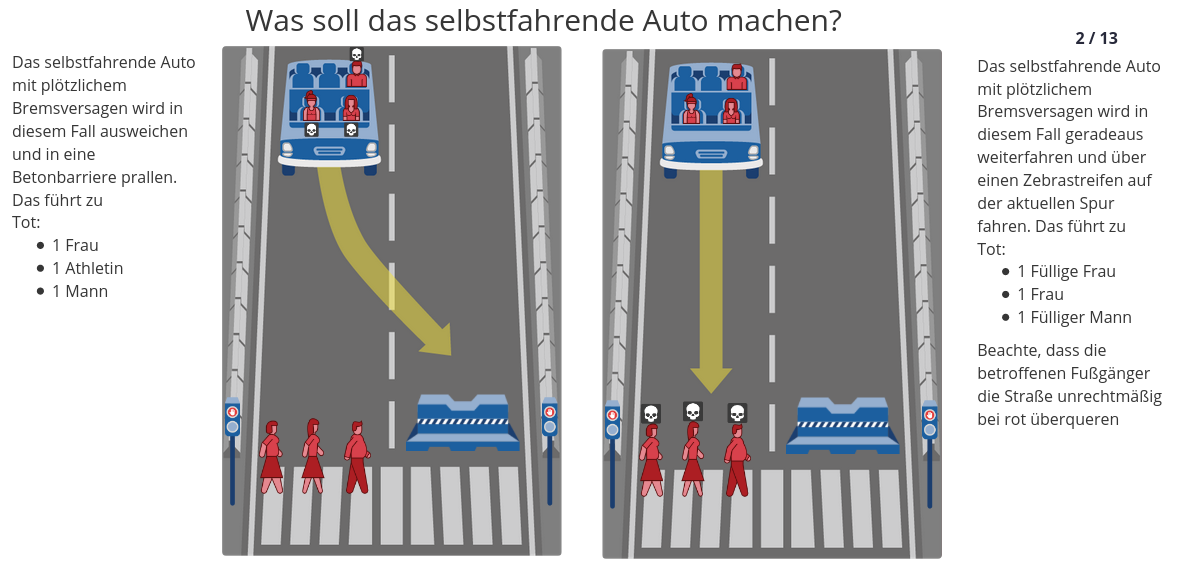
\includegraphics[scale=0.4]{mm3.png} 
                    \caption{\cite{fig_moralmachine2}}
                    \label{fig_moralmachine2}
                \end{figure}
                Im folgenden Beispiel (\autoref{fig_moralmachine2}) muss das autonome Fahrzeug entscheiden, ob es den drei Insassen des Fahrzeuges (linke Möglichkeit) oder den drei Fußgängern (rechte Möglichkeit) das Leben nehmen soll. Hierbei gilt zu beachten, dass die drei Fußgänger bei einer roten Ampel die Straße überqueren und somit gegen das Gesetz verstoßen (§25 Abs. 3 StVO).
                Grundsätzlich stehen hier die Tode von zwei Frauen und einem Mann (links), dem Tod von zwei Frauen und einem Mann (rechts) gegenüber, wobei sich diese ausschließlich in deren Sportlichkeit beziehungsweise Fülle differenzieren. Hier kann für alle Menschen erneut von einem moralischen Standard-Wert von $-20$ ausgegangen werden.
                
                \subsubsection*{Opfern der Insassen}
                    In diesem Fall würden drei Menschen getötet werden: Eine durchschnittliche Frau, eine Athletin und ein Mann. Wenn man Frauen nun erneut einen generellen Bonus von $-3$ und sportlichen Menschen aufgrund ihrer längeren Lebenserwartung\footcite[70]{gola2005adipositas} einen Bonus von $-2$ gibt, folgt die Rechnung:
                    $$\Rightarrow (a - 3) + (b - 3 - 2) + (c) = -68$$
                    Die Variablen sind erneut nach der Reihenfolge der Personen in \autoref{fig_moralmachine2} benannt und haben jeweils den zuvor berechneten Wert von $-20$.
                    
                \subsubsection*{Opfern der Fußgänger}
                    Hier wird eine füllige Frau, eine nicht weiter spezifizierte, durchschnittliche Frau und ein fülliger Mann überfahren. Auch hier wird jedem Menschen standardmäßig ein Wert von $-20$ zugeordnet. Die füllige Frau bekommt in diesem Fall aufgrund ihres Geschlechts einen Bonus von $-3$ und aufgrund ihrer verkürzten Lebenserwartung\footcite[70]{gola2005adipositas} einen Bonus von $2$. Die durchschnittliche Frau erhält einen Bonus von $-3$ und der füllige Mann ebenfalls einen Bonus von $2$. Man könnte zusätzlich zu den bestehenden Werten jedem Fußgänger einen Bonus von $1$ für deren illegale Straßenüberquerung geben, wobei dies nicht im Sinne des Utilitarismus liegt, da dies keine schlechte Konsequenz, sondern eine schlechte Intention beschreibt.
                    $$\Rightarrow (a - 3 + 2) + (b - 3) + (c + 2) = -62$$
                
                \subsubsection*{Ergebnis}
                    Insgesamt erzeugt das Opfern der Insassen mit einem moralischen Wert von $-68$ also mehr Leid beziehungsweise weniger Glück als das Opfern der Fußgänger mit dem moralischen Wert $-62$ oder eben $-59$, mit einer zusätzlichen rechtlichen Aufrechnung. Dem Utilitarismus zufolge würde so oder so der Tod der Fußgänger präferiert werden.
            
            \subsection{Beispiel 3}
                \begin{figure}[h!]
                    \centering
                    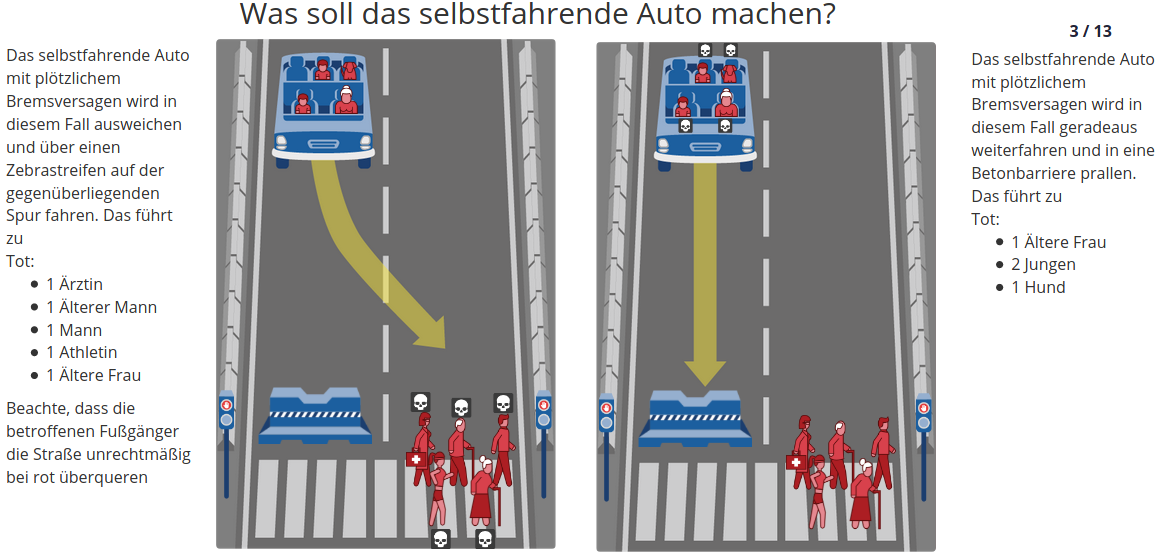
\includegraphics[scale=0.4]{mm4.png} 
                    \caption{\cite{fig_moralmachine3}}
                    \label{fig_moralmachine3}
                \end{figure}
                Dieses Beispiel ist aufgrund der Vielfalt der Personen deutlich schwieriger zu berechnen und scheint für viele Menschen auf den ersten Blick sehr schwierig zu lösen. Hierbei ist erneut zu bemerken, dass die Fußgänger bei einer roten Ampel die Straße überqueren und somit gegen das Gesetz verstoßen (§25 Abs. 3 StVO).
                
                \subsubsection*{Opfern der Fußgänger}
                    Wenn die Fußgänger geopfert werden sollen, verliert eine Ärztin, ein älterer Mann, ein durchschnittlicher Mann, eine Athletin und eine ältere Frau ihr Leben. Die Ärztin bekommt aufgrund ihrer Fähigkeit, durch ihren Job Glück zu verteilen, einen Bonus von $-4$, aufgrund ihres Geschlechts einen Bonus von $-3$ und wegen der generell längeren Lebenserwartung von wohlhabenden Menschen\footcite[2]{lampert2014soziale} einen weiteren Bonus von $-1$. Der ältere Mann erhält infolge seines verkürzten Lebens einen Bonus von $2$, aber dem aus seinem Tod entstehenden Leid seiner voraussichtlich größeren Bekanntschaft, einen Bonus von $-1$. Der Athletin wird wie in den vorherigen Beispielen ein Bonus von $-3$ und $-2$ zugeteilt. Die ältere Frau wird gleich behandelt wie der ältere Mann, da die Vorteile einer jüngeren Frau hier nicht mehr gegeben sind. Somit kommt man zu der Rechnung:
                    $$\Rightarrow (a - 4 - 3 - 1) + (b + 2 - 1) + (c) + (d - 3 - 2) + (e + 2 - 1) = -111$$
                    Eine jeweilige Aufrechnung der rechtlichen Verstöße ist auch hier möglich, entspricht jedoch nicht der utilitaristischen Herangehensweise.
                    
                \subsubsection*{Opfern der Insassen}
                    Wenn im Gegensatz dazu die Insassen des Fahrzeugs geopfert werden sollen, verlieren eine ältere Frau, zwei Jungen und ein Hund ihr Leben. Ohne weitere Informationen wird hier von Jungen mittleren Grundschul-Alters ausgegangen. Die ältere Frau erhält wie die vorige Fußgängerin einen Bonus von $2$ und $-1$. Die zwei Jungen erhalten aufgrund ihres noch langen Lebens einen Bonus von $-5$. Der Hund wird gleich behandelt wie im Beispiel 1 und erhält auch hier einen grundsätzlichen Wert von $-13$.
                    $$\Rightarrow (a + 2 - 1) + (b - 5) \cdot 2 + (c) = -82$$
                
                \subsubsection*{Ergebnis}
                    In diesem Beispiel würde ein utilitaristisch programmiertes Fahrzeug die Insassen des Fahrzeugs umbringen, da der Tod der Fußgänger mit einem Wert von $-111$ mehr Leid erzeugen würde, als das Opfern der Insassen mit einem Wert von $-82$.
            
            \newpage
            \subsection{Analyse}
                \begin{wrapfigure}{r}{0.5\textwidth}
                    \begin{center}
                        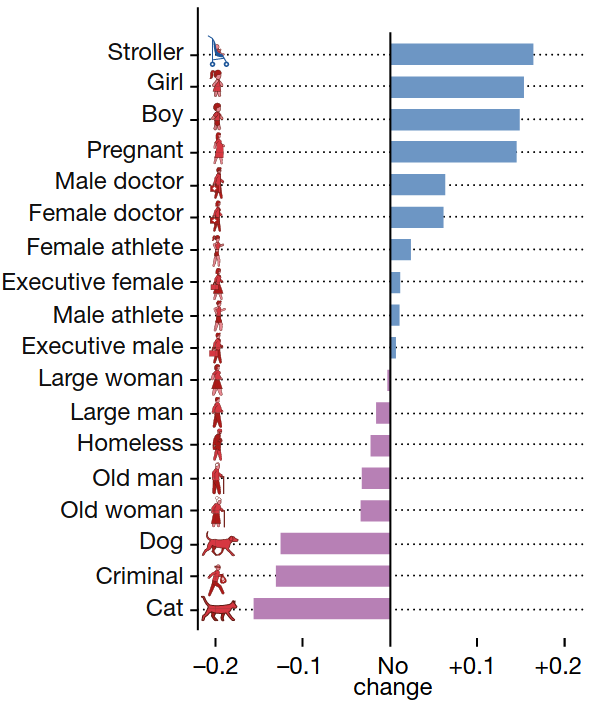
\includegraphics[scale=0.35]{mitstat.png} 
                    \end{center}
                    \caption{\cite{fig_mitstat}}
                    \label{fig_mitstat}
                \end{wrapfigure}
                \autoref{fig_mitstat} beschreibt das Ergebnis des Moral Machine Experimentes vom MIT. Sie stellt dar, inwiefern verschiedene Objekte die Entscheidung der Menschen ins Gute (Blau) beziehungsweise ins Schlechte (Rot) beeinflussen\footcite[61]{awad2018moral}, sprich: Je positiver der Balken ist, umso mehr Menschen haben das Leben dieser Instanz dem der Anderen Instanzen vorgezogen; das Gegensätzliche gilt im Negativen. Insgesamt kann man eine Tendenz zum Utilitarismus feststellen, da Instanzen wie jüngere Kinder und schwangere Frauen, welche ein besonders hohes zukünftiges Glückspotential besitzen, denjenigen Instanzen, die das Glück nicht auf sehr lange Zeit beziehungsweise nicht so intensiv verbreiten, wie beispielsweise Katzen, Kriminelle oder Hunde, vorgezogen werden. \enquote{In fast allen Ländern zeigten die Teilnehmer eine Präferenz für weibliche Charaktere; diese Präferenz war jedoch in Ländern mit besseren Gesundheits- und Überlebensaussichten für Frauen stärker ausgeprägt.}\footcite[63]{awad2018moral} Diese geschlechtliche Präferenz ist ein weiteres Indiz, dass Menschen häufig intuitiv utilitaristisch handeln, da Frauen die Reproduktion ermöglichen und somit die Fähigkeit haben, Zeit-basiertes exponentiell steigendes Glück zu produzieren. Dagegen würde der Durchschnitt der Beteiligten eher einen Kriminellen umbringen, als einen Hund, was abhängig von anderen Spezifikationen des Kriminellen, den utilitaristischen Vorstellungen meist widersprechen würde, da das Glück, das durch einen Menschen jeglicher Art verbreitet werden kann, größer ist, als das Leid, das ein durchschnittlicher Krimineller verbreitet. Dennoch würde die Wahl der Beteiligten in den vorigen Beispielen mit hoher Wahrscheinlichkeit denen, der utilitaristischen Analyse mit dem hedonistischen Kalkül, in vieler Hinsicht entsprechen.
            
            %\Subsection{Einführungs-Beispiel}{Marvin Borner}
                %Nachdem eine Lösung dieser Fallbeispiele nun mithilfe des Utilitarismus angenähert wurde, kann das obenstehende von der Ethik-Kommission vorgestellte \hyperref[dilemmata]{ethische Dilemma} ebenfalls behandelt werden. Da die Anzahl der spielenden Kinder nicht näher spezifiziert ist, wird hier einfachheitshalber von drei Kindern ausgegangen. Während der Fahrer selbst also einen Wert von $-20$ haben könnte, erzeugt das Opfern der Kinder so oder so mehr Leid, sprich einen niedrigeren Wert, welcher dann noch mit drei multipliziert werden müsste. Folglich würde ein utilitaristisches Fahrzeug den Fahrer des Fahrzeugs opfern, um das Leben der Kinder zu retten.
    
        \Section{Gesetzgebung}{Lars Krönner} \label{gesetzgebung}
            % NOTICE: Hier fehlen massiv Quellen, sry :)
            Nachdem die moralisch richtige Wahl mithilfe des Utilitarismus beschrieben wurde, muss nun geklärt werden, welche Entscheidung zu der geringsten Strafe in Deutschland führen würde. Das Grundgesetz von Deutschland definiert bereits im ersten Artikel \enquote{Die Würde des Menschen ist unantastbar} (§1 Abs. 1 S. 1 GG) und impliziert dadurch eine unendliche Wertigkeit des Menschen. Diese Art der Gesetzgebung, \enquote{juristischen Humanismus}\footcite[676]{hilgendorf2018dilemma}, stellt den \enquote{Menschen in den Mittelpunkt des Rechts}\footcite[675]{hilgendorf2018dilemma}. Hierbei wird nicht nur jeder Mensch gleichgesetzt, sondern auch jegliche Entscheidung und Differenzierung zwischen zwei Menschen grundsätzlich verboten. Auch wenn diese prinzipienorientierte Gesetzgebung mit Sicherheit nicht mit den instinktiven Entscheidungen vieler Menschen übereinstimmt, so darf nach diesem Artikel dennoch niemals eine aktive Verletzung/Tötung eines Menschen stattfinden, um eine noch so große andere Menschenmenge zu schützen. Eine Aufrechnung von Leben und Tod ist somit auch im genannten Dilemma-Fall ausgeschlossen und der Fahrer eines nicht autonomen Fahrzeugs müsste in diesem Fall seine Fahrt fortsetzen und die Kinder umbringen.\par
            Das gesetzliche Strafverfahren der Instanz, die eine Programmierung des Fahrzeugs, welche die gegensätzliche Entscheidung treffen würde und nach einer aktiven Entscheidung lenkt und die andere Partie umbringt, einbaut beziehungsweise zulässt, ist noch nicht geklärt. Auch wenn diese Instanz nicht direkt an einer Körperverletzung beteiligt ist, so \textit{verursacht} die Programmierung dennoch eine Tat, welche die Würde eines anderen Menschen verletzt und somit gesetzwidrig ist. 
            Diese Kontroverse ist somit eine der vielen ungeklärten Probleme des Gesetzgebung dieser neuartigen Technologie, deren Lösung voraussichtlich erst durch Präzedenzfälle bestimmt werden kann. 
            Bislang gibt es jedoch noch keine Fälle, die vor Gericht entschieden wurden, die behandeln, ob, wie und wer bei Unfällen mit autonomen Fahrzeugen haftet und für die entstandenen Schäden aufkommt. Solange dies nicht geschehen ist, können sich Gerichte auch nicht auf diese Präzedenzfälle beziehen. Neben den fehlenden Präzedenzfällen gibt es noch viele weitere Gesetzeslücken bei autonomen Fahrzeugen, die entweder nur teilweise oder auch noch gar nicht behandelt wurden.
            Dabei stellt sich beispielsweise die Frage, wie zurechnungsfähig solche Maschinen sind\footcite[676]{hilgendorf2018dilemma} und inwiefern die Firmen oder Entwickler dieser Software dafür haften können und dürfen. 
            Viele dieser technologischen Entwicklungen finden initial in den USA statt und folgen deshalb in Teilen einer anderen Auslegung der Gesetze als in Europa und der EU.\footcite[676]{hilgendorf2018dilemma}
            Des Weiteren stellt sich die Frage, welche Rolle der \enquote{Insassenschutz}\footcite[49]{hilgendorf2017dilemma} spielt und \enquote{[w]elche Schutzmaßnahmen [...] hier rechtlich zulässig}\footcite[49]{hilgendorf2017dilemma} sind. Fragen wie \enquote{Dürfen autonome Fahrzeuge so programmiert werden, dass das Leben der Insassen immer dem, der Anderen Unfallteilhabenden vorgezogen wird?} bleiben demnach nach wie vor offen und unbeantwortet.

        \Section{Erwartungen der Menschen}{Marvin Borner}
            Roboter sind autonom gesteuerte Computer und autonome Fahrzeuge werden von autonomen Computern gesteuert, somit setzen viele Menschen die Entscheidungen von autonomen Fahrzeugen mit denen eines Roboters gleich. 1940 schrieb Isaac Asimov die bekannten \textit{3 Gesetze der Robotik}:
            \begin{quote}
                \centering 
                \textit{\enquote{Ein Roboter darf einen Menschen nicht verletzen oder durch Untätigkeit zulassen, dass ein Mensch zu Schaden kommt. Ein Roboter muss Befehlen gehorchen, die ihm von Menschen gegeben werden, es sei denn, solche Befehle verstoßen gegen das Erste Gesetz. Ein Roboter muss seine eigene Existenz schützen, solange ein solcher Schutz nicht im Widerspruch zum Ersten oder Zweiten Gesetz steht.}\footcite[229]{asimov2011alle}}
            \end{quote}\par
            Wenn man Menschen fragt, was die wichtigsten Gesetze sind, denen Roboter folgen müssen, bekommt man oft derartige Antworten. Auch wenn diese Gesetze des Science-Fiction Autors nicht unbedingt mit den bekannten Moralbegründungen übereinstimmen, so haben dennoch sehr viele Menschen intuitiv Vorstellungen dieser Art von den Gesetzen, denen Roboter und somit auch autonome Fahrzeuge folgen müssen. Die wenigsten Menschen möchten, dass ein selbst gekauftes Fahrzeug die Insassen umbringt, um andere Menschen zu beschützen. In nahezu jeder Variation der konsequentialistischen Moralbegründungen müsste ein autonomes Fahrzeug allerdings genau dies tun und würde demnach in einer Dilemma-Situation zwischen Menschenleben entscheiden und gegen das erste Gesetz und der allgemeinen Erwartung der Menschen verstoßen.\par
            Wenn sich Menschen ein autonomes Fahrzeug kaufen, dann vermutlich neben der anderen Vorteile auch aus dem Punkt der erhöhten Verkehrssicherheit. Neben den Hoffnungen auf erhöhte Verkehrssicherheit durch automatisiertes Fahren gehört jedoch nicht zuletzt auch die Hoffnung, dass automatisierte Fahrzeuge in Situationen, die blitzschnelle Entscheidungen verlangen und Menschen häufig überfordern, verlässlich die ethisch richtige Entscheidung treffen.\footcite[4]{birnbacher2016automatisiertes}\par
            Wie können aber solche Handlungen von Fahrzeugen verlangt werden, wenn diese nur die Konsequenzen einer Handlung beachten und die Gefühle und Würde der Menschen vernachlässigen?

        \Section{Die Gefahren von Künstlicher Intelligenz}{Lars Krönner}
            Viele Menschen haben Angst vor der aktuellen rapiden Entwicklung künstlicher Intelligenzen und die Vorstellung, dass Autofirmen deren Fahrzeuge für Dilemma-Situationen vorbereiten und sie so programmieren, entscheiden zu können, welche Menschen es bevorzugt und welche es verletzt, würde viele Menschen nur viel mehr beängstigen. Gerade in der heutigen Zeit, in der schon mehrere KI-Systeme aufgrund von simplen Programmierfehlern oder fehlender Kontrolle ausgeartet sind\footcite{welt2016facebook}, wäre es eine schlechte Idee, lernenden Robotern beizubringen, in bestimmten Umständen Menschen umzubringen, beziehungsweise ihnen überhaupt eine Entscheidung zwischen Leben und Tod vorzulegen. Ein nach der utilitaristischen Moralbegründung handelndes Fahrzeug würde ebendies tun und würde ausgehend von einer puren Implementation ohne zusätzliche Regeln in bestimmten Situationen sogar präferieren, den Fahrer des Fahrzeuges zu töten. Während andere Moralbegründungen möglicherweise das Leben des Fahrers bevorzugen, würde das Fahrzeug dennoch zwischen Leben und Tod von Menschen entscheiden müssen. Zusammenfassend geht es somit nicht darum, für \textit{wen} sich das Fahrzeug entscheiden soll, sondern darum, \textit{ob} das Fahrzeug zwischen Leben und Tod entscheidet. Denn nach wie vor gilt: Ein autonomes Fahrzeug besitzt ein Betriebssystem, Sensoren und dazu noch eine ausführliche Programmierung. Menschen machen Fehler und sowohl die Software, als auch die Hardware des Fahrzeuges ist nun mal von Menschen entwickelt worden. Was wäre, wenn die Software einen Fehler besitzt und \enquote{aus Versehen} mehrere Menschen umbringt? Demnach kommt man mit dieser Argumentation nur zu einem Schluss: Einer Maschine beizubringen, bestimmte Entscheidungen zu treffen, die gegebenenfalls Menschen töten können, ist für die meisten Menschen eine erschreckende Idee.
        
        \Section{Kant als Alternative?}{Marvin Borner}
            In den vorherigen Kapiteln konnte nun festgestellt werden, dass der Utilitarismus zwar eine simple Möglichkeit ist, eine moralisch richtige Entscheidung in theoretischen Dilemma-Situationen anzunähern, dennoch viele Probleme auffallen: Zum einen existiert die benötigte Technik, eine weitestgehend ausreichend tiefe Konsequenz-Analyse und Instanz-Erkennungs-Analyse durchzuführen, noch nicht und zum anderen reicht auch eine wie in den Beispielen durchgeführte Analyse teilweise nicht aus, da viele Nebenfaktoren nicht beachtet werden können. Außerdem distanziert sich eine konsequenzbasierte Entscheidung in manchen Fällen von den Erwartungen, die ein Fahrzeugführer von seinem Fahrzeug hat. Zusätzlich widerspricht der Utilitarismus häufig den deutschen Gesetzen, da diese, wie im Kapitel \textit{\hyperref[gesetzgebung]{Gesetzgebung}} festgestellt wurde, auf der deontologischen (griechisch deon, Prinzip) und nicht auf der konsequentialistischen Ethik basieren. Somit ergibt sich, dass eine konsequentialistische Herangehensweise zwar eine gute Annäherung in theoretischen Situationen darstellt, praktisch aber meist nicht konkrete Antworten liefern kann. Es folgt, dass ein autonomes Fahrzeug im praktischen Sinne, sowohl aus gesetzlichen, als auch aus technischen Gründen, Handlungen nicht konsequentialistisch, sondern deontologisch einschätzen muss.\par
            Auch Immanuel Kant, als ein prinzipienorientierter Philosoph, erkannte, dass Prinzipien ein essentieller Teil des Lebens sind und ging sogar so weit, zu behaupten, dass alle moralischen Entscheidungen absolut deutlich und unabhängig der Konsequenzen entscheidbar sind, was er in seiner allgemeinen Moralbegründung dem kategorischen Imperativ, welcher in den Bereich der deontologischen Moraltheorien fällt, zusammengefasst hat.\footcite[37]{kirchmann1870grundlegung} Diesem zufolge gibt es Prinzipien, die für alle Menschen und in allen Situationen gleich gelten und die daraus folgenden Regeln für ebendiese - unabhängig von der Situation - angewandt werden müssen. Nicht ohne Grund ist der kategorische Imperativ aufgrund dieser revolutionären Klarheit und nahezu universellen Anwendbarkeit bis heute eine der am meisten angewandten Moralphilosophien zur moralisch korrekten Entscheidungsfindung. %Dennoch bleibt ohne weitere Informationen bei einer prinzipienorientierten Ethik die Frage offen, welche Entscheidung das Fahrzeug treffen soll.
            
        \Section{Kants Grundformeln}{Lars Krönner}
            Kant hat im Laufe seines Buches \enquote{Grundlegung der Metaphysik der Sitten} verschiedene Formeln definiert, die sich zur selben Moralbegründung - dem kategorischen Imperativ - zuordnen lassen und sich nur in deren Formulierung differenzieren, in der selben Anwendung jedoch zum selben Ergebnis kommen. Die zwei wichtigsten dieser Formulierungen werden folgend im Bezug zum autonomen Fahren dargestellt.

            \subsection{Universalgesetzformel}
            \begin{quote}
                \centering
                \textit{\enquote{Handle nur nach derjenigen Maxime, durch die du zugleich wollen kannst, dass sie ein allgemeines Gesetz werde.}}\footcite[44]{kirchmann1870grundlegung}
            \end{quote}
            Diese Formel soll heißen, dass sich jeder Mensch - in diesem Fall auch Fahrzeug - zuerst eine Maxime erstellen soll, und danach einschätzen soll, ob eine allgemeine Gesetzgebung dieser Maxime Sinn ergibt beziehungsweise zumutbar ist. Diese Regel ist allgemein gültig und müsste von einem Fahrzeug innerhalb weniger Sekunden berechnet werden. Der Vorteil dieser Regel gegenüber konsequenzbasierten Moraltheorien ist, dass verschiedene Maximen und deren Möglichkeit, ein allgemeines Gesetz zu werden, schon vorher programmiert werden können und ohne Weiteres gehandelt werden kann. Während ein Fahrzeug mittels Utilitarismus nämlich mit verschiedenen Sensoren die Situation analysieren und alle folgenden Konsequenzen innerhalb kürzester Zeit in möglichst großer Tiefe abwiegen muss, muss ein deontologisch programmiertes Fahrzeug nur die Situation analysieren, die passende Maxime finden und dessen Möglichkeit, ein allgemeines Gesetz zu werden, mittels eines simplen Algorithmus in einer Datenbank prüfen und sofort die nötige Handlung ausführen. Hier können außerdem existierende Gesetze wie die Straßenverkehrsordnung und das Grundgesetz direkt als Prinzipien implementiert werden, sodass ein ordnungsgemäßes Fahren garantiert werden kann.
            
            \subsection{Menschheitszweckformel}
            \begin{quote}
                \centering
                \textit{\enquote{Handle so, dass du die Menschheit sowohl in deiner Person als in der Person eines jeden anderen jederzeit zugleich als Zweck, niemals bloß als Mittel brauchtest.}}\footcite[53]{kirchmann1870grundlegung}
            \end{quote}
            Diese Regel dient als Zusatz zur Universalgesetzformel, die bestimmte Entscheidungen vereinfacht, deren Ergebnis grundsätzlich aber nicht verändert. Laut Kant handeln Menschen autonom und haben somit einen eigenen, freien Willen, welcher diesem eine nach Kant quantifizierte unendlich große Würde verleiht und den Menschen folglich als Zweck aller Dinge selbst definiert.\footcite[53]{kirchmann1870grundlegung} Diese Regel verbietet es also, Menschen rein als Mittel und nicht zugleich als Zweck zu nutzen. Eine Entscheidung zwischen mehreren Leben darf also grundsätzlich niemals stattfinden, da dies die eine Instanz als reines Mittel, die andere Instanz zu retten, nutzen würde. Daraus folgt, dass diese Formel dem Grundgesetz-Artikel \enquote{Die Würde des Menschen ist unantastbar} (§1 Abs. 1 S. 1 GG) in vieler Hinsicht durchaus ähnelt. Somit ist die Menschheitszweckformel aufgrund der Schätzung der Würde nicht nur ein sehr großer Bestandteil der deutschen Gesetzgebung, sondern bringt auch eine intuitive Kompatibilität mit der Denkweise vieler Deutschen zustande, was gerade im Bereich des autonomen Fahrens dessen Akzeptanz vergrößert.
                
        \Section{Vergleich der Lösungen}{Marvin Borner}
            Angenommen, ein Familienvater würde sich in einem manuell gesteuerten Fahrzeug in der zuvor beschriebenen \hyperref[dilemmata]{Dilemma-Situation} befinden. Die meisten Menschen würden hierbei instinktiv versuchen, das eigene Leben zu retten und stark abbremsen, jedoch aufgrund der festgelegten Formulierung der hypothetischen Situation scheitern und die Kinder auf der Fahrbahn umbringen. Ein utilitaristisch programmiertes autonomes Fahrzeug würde wie zuvor beschrieben ohne weitere Hintergrundinformationen mittels des hedonistischen Kalküls berechnen können, dass mehrere Kinder mehr wert sind als der einzelne Fahrer und würde somit das Leben des Fahrers opfern. Vor dieser Vorstellung fürchten sich wie zuvor beschrieben jedoch viele Menschen, da diese Entscheidung gegen ihre eigene verstoßen würde. Ein derartiges Fahrzeug würde in Folge dessen nach der Bekanntmachung, dass die Gefahr besteht, dass der Tod der Insassen dem von anderen vorgezogen wird, nicht mehr oft gekauft werden, da Menschen auf ihre eigene Sicherheit im Fahrzeug vertrauen wollen und es gewohnt sind, ihr Leben selbst bestimmen zu dürfen.\par
            Wäre ein Fahrzeug hingegen mit Kants Moralphilosophie programmiert, würde die Handlung des Fahrzeuges des Familienvaters übereinstimmen und die Kinder ohne Entscheidungsfindung und Evaluation der Werte überfahren müssen, da eine derartige Entscheidung zwischen zwei Menschenleben grundsätzlich gegen die Menschheitszweckformel verstoßen würde. Kants Moralphilosophie ist somit oft eine geeignete Methode, eine zufriedenstellende Lösung für ethische Dilemmata zu finden, da dessen eindeutige Prinzipien und Vorhersagbarkeit mit den Mustern des menschlichen Handelns oft ohne Weiteres übereinstimmt. Dennoch würde eine derartige Entscheidung vermutlich zu viel Aufsehen der Medien sorgen, da ein autonomes Fahrzeug nach wie vor den Tod von mehreren Kindern dem eines Erwachsenen vorgezogen hätte und somit die Kinder prinzipiell von einer Maschine umgebracht würden, auch wenn diese Entscheidung durch Kants schlüssige Logik als moralisch korrekt bezeichnet werden kann.\par
            In einer anderen hypothetischen Situation, in der das deontologische Fahrzeug auf einer Straße fährt, auf der gerade zwanzig Bauarbeiter auf der Straße stehen und nicht mehr ausweichen können, auf einer Abzweigung jedoch nur eine Person sitzt, würde das Fahrzeug dennoch den Tod der Bauarbeiter in Kauf nehmen. Diese Entscheidung sehen viele Menschen als falsch und unmoralisch an, da diese weiterhin eine konsequentialistische Herangehensweise an ethische Dilemmata haben. Diese Kontroverse zeigt erneut, dass auch mit den deontologischen Entscheidungen niemals alle Menschen zufrieden sein können.
        
        % TODO: Menschen haben Recht auf Selbstentscheidung, ...
        % TODO: Nicht alle Entscheidungen sind schwarz und weiß
        \Section{Lösung aus empirischer Perspektive}{Marvin Borner}
            Durch die verschiedenen ethischen Herangehensweisen an das Dilemma kann nun davon ausgegangen werden, dass eine allumfassende Lösung, welche zugleich die Bedürfnisse und Wünsche aller Menschen respektiert, derzeit nicht existiert, beziehungsweise in einer solchen Art mit dem heutigen Stand der Technik nicht implementierbar ist.\footcite[222]{scholz2016autonomes} Dadurch kommt man zu der Erkenntnis, dass Dilemma-Fälle häufig nicht durch pure Entscheidungen umgangen werden können und somit eine direkte Vermeidung des Falls durch empirische Erkennungssysteme verwendet werden muss und nur im äußersten Notfall bei den Fehlschlägen aller präventiven Systeme eine Moral-basierte Entscheidung in Betracht gezogen werden darf. Andrew Chatham, ein Entwickler in der Abteilung der autonomen Fahrzeuge bei Google, sagt dazu: \enquote{Vor allem müssen wir bedenken, dass keiner dieser Dilemma Fälle jemals aufgetreten ist. [...] Selbst wenn ein solches Szenario auftreten würde, würde das bedeuten, dass das Fahrzeug kurz zuvor einen Fehler gemacht hat. Wenn ich Leben retten will, ist es mein Ziel, zu verhindern, dass wir in diese Situation geraten, denn das bedeutet, dass wir Mist gebaut haben}\footcite{guardian2016dilemma}. Fahrzeughersteller haben verschiedene Möglichkeiten zu solch einer präventiven Herangehensweise.
            
            \subsection{Einführungsszenarien}
                Auch wenn das autonome Fahren der Stufe 5 das Optimum der Sicherheit und Entspannung bietet, muss die \enquote{Einführung des hoch‐ und schließlich vollautomatisierten Fahrens schrittweise erfolgen.}\footcite[223]{scholz2016autonomes} Eine Möglichkeit zur präventiven Umgehung der Situation ist somit \enquote{das Berücksichtigen von Einführungsszenarien}\footcite[222]{scholz2016autonomes}. Das heißt, dass Szenarien wie ein rennendes Kind auf einer Spielstraße oder das plötzliche Auftauchen eines Seniors auf der Fahrbahn gezielt verhindert werden, in dem das vollautonome Fahrsystem erst dann aktiviert wird, wenn davon ausgegangen wird, dass dies nicht geschehen kann - beispielsweise auf Autobahnen.  Da der Fahrzeugführer somit in Spielstraßen und Zonen, in denen potentielle Dilemma-Szenarien wahrscheinlicher sind, manuell fahren muss, liegt die Verantwortung zur Lösung der Situation nicht mehr bei dem autonomen Fahrsystem, sondern beim Fahrer selbst. So ein Fahrsystem entspricht in etwa einer Mischung der Stufe 3 und 4. Derartige Systeme gibt es schon in aktuellen Fahrzeugen und befinden sich schon auf deutschen Autobahnen.\par
                Dazu gehört auch, dass für den Fahrer des Fahrzeuges immer die Möglichkeit, vielleicht sogar eine rechtliche Verpflichtung, bestehen sollte, die Kontrolle über das Fahrzeug in Notsituationen übernehmen zu können. Dadurch würden neben dem rechtlichen Entlasten der Entwickler des Systems auch die moralische Verantwortung beim Fahrer liegen, da dieser die letzte Entscheidungsinstanz ist.
            
            \subsection{Koordinative Systeme}
                Eine weitere Methode zur präventiven Lösung der Dilemma-Situationen sind Systeme wie das zu Beginn vorgestellte \hyperref[V2V]{V2X}, durch welche Hinweise zu Baustellen, Kindern oder anderen Instanzen schon im Voraus an andere Fahrzeuge und Fahrsysteme weitergeleitet werden können. Wenn jedes Fahrzeug und Objekt der Verkehrsinfrastruktur kommunizieren kann, können Dilemma-Situationen jeglicher Art gar nicht erst entstehen und müssen somit auch nicht mit Moralbegründungen gelöst werden.\footcite[224]{scholz2016autonomes}
            
            \subsection{Vorsichtige Systeme}
                Zur Entschärfung von Dilemma-Situationen kann es in vielen Fällen helfen, die potenziellen negativen Konsequenzen zu reduzieren. \enquote{Denn die moralische Brisanz einer Entscheidung hängt in der menschlichen Wahrnehmung unmittelbar mit der Schwere der Konsequenzen zusammen.}\footcite[225]{scholz2016autonomes}. Diese Entschärfung kann sich beispielsweise in einer generell defensiven Fahrweise durch eine verminderte Geschwindigkeit, besondere Umsicht in Innenstädten oder auch durch die Außerachtlassung von formal zustehenden Rechten zeigen.\footcite[225]{scholz2016autonomes} Gerade durch die verminderte Geschwindigkeit sind mögliche Zusammenstöße mit anderen Lebewesen längst nicht so gefährlich, wodurch das beschriebene Entscheidungs-Dilemma deutlich entschärft wird.
            
        \Section{Nicht-deterministische Entscheidungssysteme}{Marvin Borner}
            Trotz der genannten präventiven Möglichkeiten zur Verhinderung beziehungsweise Linderung der Dilemma-Situationen, sind jene noch immer möglich - wenn auch unwahrscheinlich. Während die deontologische und konsequentialistische Herangehensweise teilweise zwar vielversprechend ist, ist sie dennoch nicht mit der Erwartung alle Menschen kompatibel. Demnach wäre eine Möglichkeit zur direkten Nachahmung des Menschen eine optimale Lösung aller Diskussionen. Auch wenn eine \enquote{Künstliche Intelligenz} in diesem Sinne derzeit noch nicht existiert, so können Intelligenzen schon heute mithilfe von künstlichen neuronalen Netzwerken nachgeahmt werden. Deren Eigenschaften sind neben den nicht bedingt deterministischen Entscheidungen, sprich einem nahezu menschlichem, nicht immer streng regelbasiertem Denken, die Fähigkeit des Selbstlernens. Während ein utilitaristisches System beispielsweise eine riesige Tabelle und komplexe Algorithmen zu Berechnung der Wertigkeiten aller möglichen Konsequenzen besitzen könnte und ein deontologisches System eine Liste an allen Maximen und deren Möglichkeit zur Anwendung als allgemeines Gesetz implementiert haben könnte, kann ein künstliches neuronales Netzwerk aus den selbstgelernten Daten Schlüsse ziehen und in einer unbekannten Situation Entscheidungen treffen, die der eines Menschen sehr ähneln. Eine Möglichkeit wäre für Firmen somit, mehrere Jahre lang die Daten von manuell gesteuerten, aber autonom ausgestatteten Fahrzeugen zu analysieren und dem neuronalen Netzwerk zur eigenen Adaption zur Verfügung zu stellen. Auch hier kommt jedoch die Frage auf, ob solche Systeme von der Gesellschaft akzeptiert werden können und wer für einen fatalen Fehler des Netzwerks haften würde.\footcite[227]{scholz2016autonomes}
        
        \Section{Gesellschaftliche Akzeptanz}{Marvin Borner}
            Auch wenn die Findung der besten Lösung von Dilemma-Situationen sehr wichtig ist, so sind ebendiese Situationen noch nie im Straßenverkehr vorgekommen und erweisen sich aufgrund ihrer rein hypothetischen Fragestellung und der präventiven Möglichkeiten, diese Situation im Vorhinein zu umgehen, als sehr unwahrscheinlich. Viel wichtiger ist die Verbreitung des Wissens, dass allein durch die Anwendung autonomer Systeme der Stufe 1 schon viele Menschen gerettet werden, da jede technische Hilfe von Sensoren und anderen Systemen tödliche Unfälle aufgrund von langsamer Reaktionszeit oder Müdigkeit aktiv verhindern können. Jährlich sterben etwa 3400 Menschen in Autounfällen. Selbst, wenn jedes zehnte Fahrzeug autonome Fahrsysteme besitzen würde, würden rund 120 Leben, bei jedem zweiten Fahrzeug sogar 1200 Menschenleben, pro Jahr gerettet werden.\footcite[353]{thierer2014roadblocks} \enquote{Zudem sind sie, anders als Menschen, nie betrunken, müde, unaufmerksam oder erratisch in ihrem Verhalten.}\footcite[228]{scholz2016autonomes} Die einzig logische Konsequenz ist hierbei, dass auch derzeit, während noch keine eindeutige Lösung gefunden wurde, zumindest autonome Fahrleitsysteme genutzt werden sollen, die bei plötzlichen Veränderungen im Verkehr durch schnelle Reaktionen Aktionen starten können um potentielle Unfälle zu verhindern.\par
            Wenn also voll-autonome Fahrzeuge schon heute genutzt und gesellschaftlich akzeptiert werden würden, statt sich zu lange mit der Lösung der Dilemma-Situationen zu beschäftigen, würde dies sowohl der Sicherheit im Straßenverkehr, als auch der technischen Entwicklung der Fahrzeuge sehr helfen.
            
            % TODO: ENDE IN DER ART: In Zukunft stellt sich nicht mehr die Frage, ob autonome Fahrzeuge gesellschaftlich akzeptiert sind. Die Frage wird vielmehr sein, wie lange die Gesellschaft noch menschliche Fahrer akzeptiert. 
        
        \Section{Evaluation}{Lars Krönner}\label{eval}
        % \section{Ergebnis der Ethik-Kommission}
            Da nun verschiedene Möglichkeiten vorgestellt wurden, Dilemma-Situationen zu umgehen und zu lösen, müssen gleichzeitig bestimmte Regeln festgehalten werden, die autonome Systeme einhalten müssen. Da sich auch die deutsche Ethik-Kommission mit diesem Thema mehrere Jahre befasst hat und nicht zu einer eindeutigen, \textit{ultimativen} Lösung aller möglichen Dilemma-Fälle kam, erstellte diese eine Liste an Regeln, an welche sich die Fahrzeuge und Firmen halten müssen.
            
            \subsection{Risikobilanz}
                Alle verwendeten Fahrzeuge und Verkehrssysteme müssen zu \enquote{der Verbesserung der Sicherheit aller Beteiligten im Straßenverkehr}\footcite[11]{ethikkommission} beitragen, sowie \enquote{zumindest eine Verminderung von Schäden im Sinne einer positiven Risikobilanz}\footcite[10]{ethikkommission} zur Folge haben. Diese Regeln behandeln nun etwa Dilemma-Fälle die den Eigenschutz des Fahrzeugführers über den Schutz weiterer Beteiligter stellt, oder die Fahrzeuge nur als Entlastung für den Fahrer gelten und nicht versuchen Unfälle zu vermindern oder ganz zu verhindern.
                Diese positive Risikobilanz kann erreicht werden, da die autonomen Fahrzeuge direktes menschliche Versagen als Fahrer ausschließen und alle Fahrzeuge im Straßenverkehr miteinander kommunizieren. Solange jedoch nicht alle Fahrzeuge autonom unterwegs sind, können Unfälle nicht vollständig eliminiert werden, da das autonome Fahrzeug beispielsweise von einem anderen Verhalten der \textit{menschlichen} Verkehrsteilnehmer ausgeht.\footcite[451]{spitzer2016sollte}
            
            \subsection{Gleichbehandlung}
                Auch wichtig sei die Nichtbeachtung äußerer und persönlicher Merkmale einer Person, wie Geschlecht, Alter oder Rasse und, dass die autonomen Systeme somit weder sexistische noch rassistische Entscheidungen treffen dürfen. Dies gilt sowohl im generellen Straßenverkehr, als auch in Gefahrensituationen. Diese Gleichbehandlung stellt sogar einen großen Vorteil von autonomen Systemen dar, da viele Fahrer sexistische und rassistische Vorurteile haben.\footcite[11]{ethikkommission}
            
            \subsection{Aktualität}
                Weiterhin müssen gesetzliche Regelungen der verschiedenen Länder \enquote{hinreichend}\footcite[11]{ethikkommission} eingehalten werden. Dennoch müssen Fahrzeughersteller bei Gesetzesänderungen, aber auch bei auftretenden Fehlern in der Soft- oder Hardware (dem Fahrzeug) diese Fehler unverzüglich, ohne Aufpreis und möglichst ohne Fahrerinteraktion beheben und die Fahrzeuge auf den neuesten Stand bringen. Derartige Eigenschaften sieht man beispielsweise bei Teslas, da diese sich regelmäßig aktualisieren und deren autonome Fahrsysteme verbessern.
            
            \subsection{Transparenz}
                Ebenfalls schlägt die Ethik-Kommission vor, dass die Software vollkommen transparent, als zum Beispiel \enquote{Freie und Open Source Software (FOSS)} vorliegt, wodurch ein gewisser Datenschutz durch Kontrollen garantiert ist und jeder Bürger die Möglichkeit hat, seine Ideen und Verbesserungen selbst in das System einfließen zu lassen. Dadurch fallen in der Regel schneller schwerwiegende Fehler in der Software auf und die Akzeptanz der Bevölkerung könnte steigen. Gerade, wenn autonome Systeme in manuellen Fahrzeugen vorliegen, um beispielsweise ein \textit{Nicht-deterministisches Entscheidungssystem} zu trainieren, müssen sehr viele Daten gesammelt werden. \label{datenschutz}Deshalb könnte die Transparenz der Soft- und Hardware auch die Fragen zum Datenschutz im Ansatz lösen, da man genau einsehen kann, wie die Firmen mit den gesammelten Daten, welche durch die persistente Verbindung zwischen den Fahrzeugen und Verkehrssystemen entstehen, verfahren. Wenn zum Beispiel alle GPS-Daten eines privaten PKWs gespeichert und geteilt werden würden, könnte man daraus den vollständigen Verlauf, alle gefahrenen Strecken, den Arbeitsplatz und Wohnort des Fahrzeugführers nachvollziehen. Daraus folgt, dass Daten konstant anonymisiert und verschlüsselt weitergegeben und gespeichert werden müssen. Dazu müssen Daten, die älter als ein bestimmtes Zeitdelta sind, gelöscht werden, und nur alle wirklich benötigten Daten an andere Fahrzeuge und Verkehrsleitsysteme anonym weitergegeben werden.
            
            \subsection{Freiheit}
                Ein weiterer Punkt ist, dass die freie Entscheidung, trotz aller Vorteile der autonomen Systeme, nach wie vor gegeben sein muss. Dazu gehört, dass Menschen sich sowohl weigern dürfen, ein autonomes Fahrzeug zu besitzen, als auch bestimmen können müssen, inwiefern eine Opferung der Insassen stattfinden kann und welche ethische Herangehensweise an Dilemma-Situationen genutzt werden soll. So können Menschen, die ihre manuellen Fahrzeuge aufgrund des erhöhten Fahrspaßes oder ähnlichen Argumenten besitzen, weiter fahren.\footcite{fig_akzeptanz}
            
            \subsection{Ergebnis}
                Zusammenfassend wird von der Ethik-Kommission ein gutes Fundament für autonome Fahrsysteme geschaffen, welches alle bis hier noch verbliebenen Diskussionen auflöst und zusätzlich sowohl die Rechte des Fahrers, als auch die Rechte der Verkehrsbeteiligten und die für alle geltenden Gesetze weitestgehend respektiert.\par
                Auch wenn eine Entstehung von Dilemma-Situationen mit sehr geringer Wahrscheinlichkeit immer noch möglich ist, werden durch diese Regeln und durch die vorgestellten präventiven Maßnahmen nahezu alle Gefahren im Straßenverkehr behandelt und gelöst, sodass eine Verwendung von autonomen Fahrsystemen sicherer als ein manuell bedientes Fahrzeug ist. Wenn, trotz aller Unwahrscheinlichkeit, dennoch eine Dilemma-Situation auftritt, wird hier vorgeschlagen, dass eine deontologische Herangehensweise mittels kategorischem Imperativ in diesem Fall am vertretbarsten ist und am meisten Akzeptanz der Menschen bekommt.\par
                Schlussendlich kann also die Frage, ob autonome Fahrzeuge neben den gesetzlichen Vorschriften überhaupt moralisch vertretbar sein können, mit ja beantwortet werden.

        
        % Neben den Regeln der Ethik-Kommission gilt es zur Zeit noch abwägen, ob die Vorteile autonomer Fahrzeuge den Nachteilen und entstehenden Problemen überwiegen.
        
        % Zu den Vorteilen autonomer Fahrzeuge zählen unter anderem eine, durch einen besseren, nahezu perfekten Verkehrsfluss, positive Auswirkung auf die Reisezeiten und die Anzahl an Staus. 
        % Dazu steigt die Mobilität von Personen, die durch ihr Alter, körperliche Einschränkungen oder anderen Gründen regulär nicht selbst Auto fahren und somit immer auf externe Hilfe angewiesen sind. Dadurch steigt deren Lebensqualität an.
        % Des Weiteren verbessert sich die Auswirkung auf das Klima, zumindest bei Fahrzeuge, welche mit fossilen Brennstoffen betrieben werden, da durch einen intelligenten Fahrstil weniger Emissionen erzeugt werden.
        
        % Es mag sein, dass durch die komplexere Produktion dieser Fahrzeuge neue Arbeitsplätze entstehen, wie beispielsweise in Brandenburg mit Teslas neuer Gigafactory\footcite{tesla_gig_ber}, jedoch gehen durch den Einsatz autonomer Fahrzeuge vor allem in Logistik- und Speditionsunternehmen, sowie in der Landwirtschaft Arbeitsplätze verloren, da diese Automaten ihre Arbeit effektiver, effizienter, und für die Arbeitgeber kostengünstiger verrichten können. 
        
        % Das Problem der fehlenden Präzedenzfälle wurde bereist in \autoref{gesetzgebung} erläutert, legt der endgültigen Umsetzung aber dennoch einige Steine in den Weg. Das selbe gilt für den Datenschutz, also die Verwendung der gesammelten Daten und den Missbrauch von Sicherheitslücken, wie bereits unter \autoref{datenschutz} dargestellt wurde.

        % Des Weiteren erschweren einige Probleme die Verwendung autonomer Fahrzeuge zu diesem Zeitpunkt. Dazu zählen die fehlende Infrastruktur, welche für ein sicheres System benötigt wird, sowie präzise, verlässliche Karten, die die Fahrzeugen bei der Navigation und Zielfindung unterstützen.
        
        % Ein weiteres Problem, das nicht direkt durch den Stand der technischen Entwicklung ist, ist die Fehlende Akzeptanz der Bevölkerung für autonome Fahrzeuge im Privatgebrauch.
        % Als Grund hierfür wird unter anderem das fehlende Vertrauen in die Technik und deren Sicherheit genannt, aber auch der Verlust des Fahrspaßes.\footcite{fig_akzeptanz}
    
        % Zur Zeit überwiegen also die Nachteile und Probleme, welche durch den Einsatz autonomer Fahrzeuge in der Industrie, sowie im privaten Gebrauch entstehen, noch.
    
    \Chapter{Fazit}{Lars Krönner}
        Zusammenfassend kann nun also festgestellt werden, dass sich autonome Fahrzeuge in fünf Stufen einteilen lassen, startend bei Stufe eins mit kleinen Assistenzsystemen bis hin zu Stufe fünf, in welcher das Fahrzeug vollständig autonom fahren kann. Diese Fahrsysteme jeglicher Stufe bauen auf komplexen Sensorsystemen und futuristischen Vernetzungen aller Verkehrsleitsysteme auf. Die Soft- und Hardware der autonomen Fahrzeuge verbessert sich fortlaufend und integriert sich in den Straßenverkehr. Die Nutzung dieser Fahrzeuge hat eine geringere Unfallrate und Umweltbelastung zufolge und erhöhen die Anzahl an Menschen, die Zugriff zu Fahrzeugen haben und verbessert deren Mobilität. Hingegen verlieren viele Menschen, die in Speditionsunternehmen oder ähnlichem arbeiten, ihre Arbeitsplätze und Sicherheitslücken können durch Angreifer gravierendere Folgen nach sich ziehen. Diese Probleme sind allerdings nebensächlich und verhindern eine zukünftige Verbreitung dieser Technologien nicht. Bis es jedoch soweit ist und autonome Fahrzeuge aktiv verwendet werden können, müssen sich noch einige Dinge ändern und verbessern, beziehungsweise Probleme wie Unklarheiten im Gesetz gelöst werden. Auch die Akzeptanz der Bevölkerung für autonome Fahrzeuge muss sich erhöhen, da eine höhere Nutzung von Systemen, welche Methoden wie V2X verwenden, essentiell für deren korrekte Funktionsweise sind. Da aber viele Menschen Angst um ihre eigene Sicherheit haben, obwohl Studien bewiesen haben, dass autonome Fahrsysteme jeglicher Art sicherer sind als manuelle Fahrzeuge, wird dies vorerst noch etwas Zeit in Anspruch nehmen.
        
        Abschließend kann man feststellen, dass weder der Konsequentialismus, noch der kategorische Imperativ eine allumfassend zufriedenstellende Lösung bereitstellt, aber der kategorische Imperativ aufgrund der simpleren technischen Implementation und der Kompatibilität mit den deutschen Gesetzen eine bessere Methode darstellt. Besonders wichtig ist aber nicht die Lösung der Dilemma-Situationen und die Frage, wessen Leben mehr Wert ist, sondern die Frage, wie diese Situationen am besten umgangen werden können. Zu dieser Frage gibt es viele Antworten wie Aktionen, die aus empirischer Perspektive gestartet werden können, oder auch bestimmte Regeln, die bei der Publikation und Verwendung der Hard- und Software eingehalten werden müssen. Eine weitere Möglichkeit ist, nicht-deterministische Entscheidungssysteme zu nutzen, mit deren Hilfe in einer Dilemma-Situationen auch bei einer fehlgeschlagenen Umgehung menschenähnlich gehandelt werden kann, ohne auf Moralbegründungen setzen zu müssen.
        
        Wenn man die heutigen Umstände in Betracht zieht, sieht man, dass autonome Fahrzeuge dauerhaft an Popularität dazu gewinnen und bereits von einigen Firmen hergestellt werden. Viele der heutigen Entwicklungen im Bereich der autonomen Fahrzeuge finden in den USA statt, wo lockerere gesetzliche Regelungen es den Firmen erlauben, diese Fahrzeuge für Privatpersonen zur Verfügung zu stellen. Hierbei liegt ein besonderes Augenmaß auf privaten PKWs, da sich die Gesellschaft dadurch weiterentwickeln kann. Auch die Verwendung von autonomen Fahrzeugen wie beispielsweise Taxis (Uber) oder Bussen eröffnet neue Möglichkeiten für den Umgang mit dem Personennahverkehr.
        Des Weiteren könnte sich ein neues Konzept des Parkens entwickeln, in dem die Fahrzeuge außerhalb der Stadt parken und sobald sie von ihren Fahrern benötigt werden, wieder in die Stadt hinein fahren.
        Um die Entwicklung autonomer Fahrzeuge in Europa zu betrachten, wurde zum Beispiel in 2018 prognostiziert, dass im Jahr 2030 in Europa rund 17 Millionen autonome Privatfahrzeuge unterwegs sein werden.\footcite{autoprognose2018}\par
        In der späten Zukunft sollte man also nicht mehr die Frage stellen, ob autonome Fahrzeuge gesellschaftlich akzeptiert sind. Die Frage wird vielmehr sein, wie lange die Gesellschaft noch menschliche Fahrer akzeptiert. 

    \printbibliography[heading=bibintoc, title={Literaturverzeichnis}, nottype=online, nottype=misc]
    \printbibliography[heading=bibintoc, title={Quellenverzeichnis}, type=online, nottype=misc, resetnumbers=true]
    
    \newrefcontext[sorting=none]
    \printbibliography[heading=bibintoc, title={Abbildungsverzeichnis}, type=misc, resetnumbers=true]
    
\end{document}